%% Proyecto.tex
%% 2020/06/08
%% por Juan Pablo Mora
%% 
%% Proyecto que demuestra soluciones graficadas numéricamente para la
%% ecuación de Laplace
%%

\documentclass[10pt,journal,compsoc]{IEEEtran}

\ifCLASSOPTIONcompsoc
  % IEEE Computer Society needs nocompress option
  % requires cite.sty v4.0 or later (November 2003)
  \usepackage[nocompress]{cite}
\else
  % normal IEEE
  \usepackage{cite}
\fi

\usepackage{listings}


\usepackage[pdftex]{graphicx}
% declare the path(s) where your graphic files are
\graphicspath{images/}
% and their extensions so you won't have to specify these with
% every instance of \includegraphics
\DeclareGraphicsExtensions{.png}

\usepackage{amsmath}
% A popular package from the American Mathematical Society that provides
% many useful and powerful commands for dealing with mathematics.
%
% Note that the amsmath package sets \interdisplaylinepenalty to 10000
% thus preventing page breaks from occurring within multiline equations. Use:
\interdisplaylinepenalty=2500
% after loading amsmath to restore such page breaks as IEEEtran.cls normally
% does. amsmath.sty is already installed on most LaTeX systems. The latest
% version and documentation can be obtained at:
% http://www.ctan.org/pkg/amsmath

% correct bad hyphenation here
\hyphenation{op-tical net-works semi-conduc-tor}


\begin{document}
%
% paper title
% Titles are generally capitalized except for words such as a, an, and, as,
% at, but, by, for, in, nor, of, on, or, the, to and up, which are usually
% not capitalized unless they are the first or last word of the title.
% Linebreaks \\ can be used within to get better formatting as desired.
% Do not put math or special symbols in the title.
\title{Soluciones de la Ecuación de Laplace}


\author{Juan~Pablo~Mora,~\IEEEmembership{Estudiante,~UVG}% <-this % stops a space
\IEEEcompsocitemizethanks{\IEEEcompsocthanksitem Thanks to Mr. Siba Prasad for all his help
during the course.}}

% The paper headers
\markboth{Teoría Electromagnética Sección~20, Proyecto~1, Mayo~2020}%
{Soluciones de la Ecuación de Laplace}
% The only time the second header will appear is for the odd numbered pages
% after the title page when using the twoside option.
% 
% *** Note that you probably will NOT want to include the author's ***
% *** name in the headers of peer review papers.                   ***
% You can use \ifCLASSOPTIONpeerreview for conditional compilation here if
% you desire.

\IEEEtitleabstractindextext{%
\begin{abstract}
Soluciones numéricas a la Ecuación de Laplace
\end{abstract}

% Note that keywords are not normally used for peerreview papers.
\begin{IEEEkeywords}
IEEE, IEEEtran, journal, \LaTeX, paper, Laplace equations.
\end{IEEEkeywords}}


% make the title area
\maketitle


% To allow for easy dual compilation without having to reenter the
% abstract/keywords data, the \IEEEtitleabstractindextext text will
% not be used in maketitle, but will appear (i.e., to be "transported")
% here as \IEEEdisplaynontitleabstractindextext when the compsoc 
% or transmag modes are not selected <OR> if conference mode is selected 
% - because all conference papers position the abstract like regular
% papers do.
\IEEEdisplaynontitleabstractindextext
% \IEEEdisplaynontitleabstractindextext has no effect when using
% compsoc or transmag under a non-conference mode.



% For peer review papers, you can put extra information on the cover
% page as needed:
% \ifCLASSOPTIONpeerreview
% \begin{center} \bfseries EDICS Category: 3-BBND \end{center}
% \fi
%
% For peerreview papers, this IEEEtran command inserts a page break and
% creates the second title. It will be ignored for other modes.
\IEEEpeerreviewmaketitle



\IEEEraisesectionheading{\section{Introducción}\label{sec:introduction}}
% Computer Society journal (but not conference!) papers do something unusual
% with the very first section heading (almost always called "Introduction").
% They place it ABOVE the main text! IEEEtran.cls does not automatically do
% this for you, but you can achieve this effect with the provided
% \IEEEraisesectionheading{} command. Note the need to keep any \label that
% is to refer to the section immediately after \section in the above as
% \IEEEraisesectionheading puts \section within a raised box.




% The very first letter is a 2 line initial drop letter followed
% by the rest of the first word in caps (small caps for compsoc).
% 
% form to use if the first word consists of a single letter:
% \IEEEPARstart{A}{demo} file is ....
% 
% form to use if you need the single drop letter followed by
% normal text (unknown if ever used by the IEEE):
% \IEEEPARstart{A}{}demo file is ....
% 
% Some journals put the first two words in caps:
% \IEEEPARstart{T}{his demo} file is ....
% 
% Here we have the typical use of a "T" for an initial drop letter
% and "HIS" in caps to complete the first word.
\IEEEPARstart{E}{l} objetivo de este articulo es demostrar el comportamiento
de potenciales eléctricos resolviendo la Ecuación de Laplace con condiciones de
frontera de Dirichlet.
\\\\
El documento consiste en los ejercicios asignados y su respectiva solución,
la cual será mostrada como un grafico en 3D o un mapa de calor en 2D el cual se
calcula utilizando el método analítico y el "truco de Fourier" para la resolución
de ecuaciónes diferenciales parciales.
\\\\
Adicionalmente en el apéndice A se escribe sobre el método de resolución y sobre 
las formas alternativas con las que se puede calular la misma solución.
\hfill mds
 
\hfill Junio 7, 2020

\subsection{Ecuación de Laplace en coordenadas rectangulares}

\subsubsection{Tubería rectangular}
Una tubería rectangular recta se extiende infinitamente a lo largo del eje \(z\).
Sus paredes se encuentran en los planos \(x=0,y=0,x=a\) y \(y=b\).
Los planos \(y = 0\) y \(y = b\) se encuentran aterrizados, mientras que los planos
\(x = 0\) y \(x = a\) se encuentran a potenciales \(g(y)\) y \(h(y)\) respectivamente.
\\\\
Determine el potencial eléctrico dentro dentro de la tubería bajo las siguientes condiciones:
\(g(y) = 0, h(y) = tan^{-1}(y/a)\)
\\

\subsubsection{Condiciones iniciales del problema}

Para empezar, escogemos un valor arbitrario para a y b, por simplicidad usamos \(a = b = 35 \)
y configuramos \(h(y) = tan^{-1}(y/a) \quad 0\leq y \leq a \)
el resultado del potencial y el campo vectorial en \(n = 20\) se puede ver en la grafica \ref{arctan-n20}
y las gráficas de menores iteraciones incluyendo las condiciones iniciales y la densidad de carga
se encuentran en la figura \ref{arctan-iterations}.
Para configurar las condiciones iniciales en el código utilizamos
\begin{lstlisting}
  T[:,-1] = np.arctan(y/y[-1])
\end{lstlisting}

\begin{figure}
  \centering
  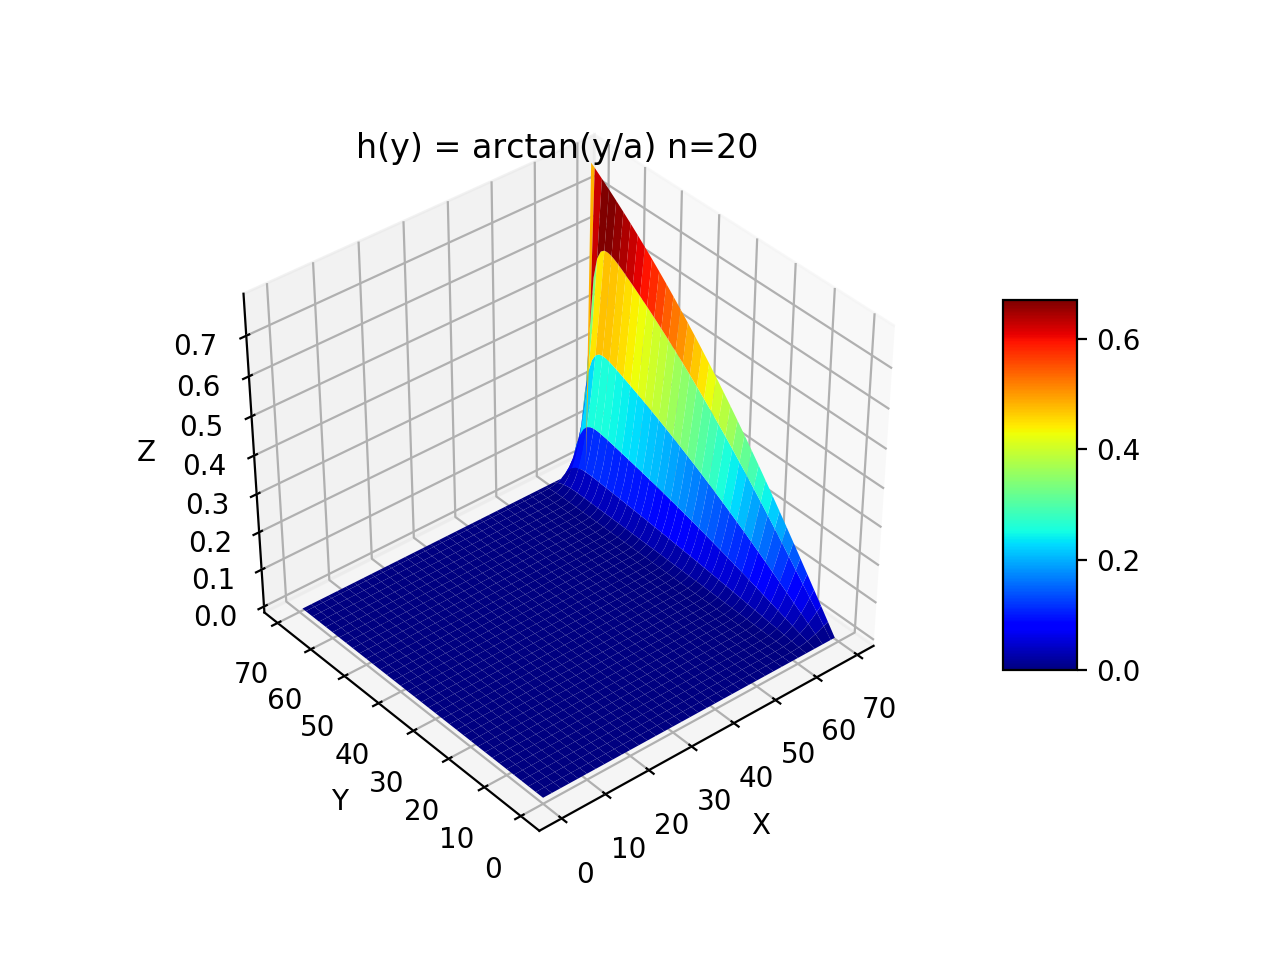
\includegraphics[width=2.8in]{images/arctan-n20}
  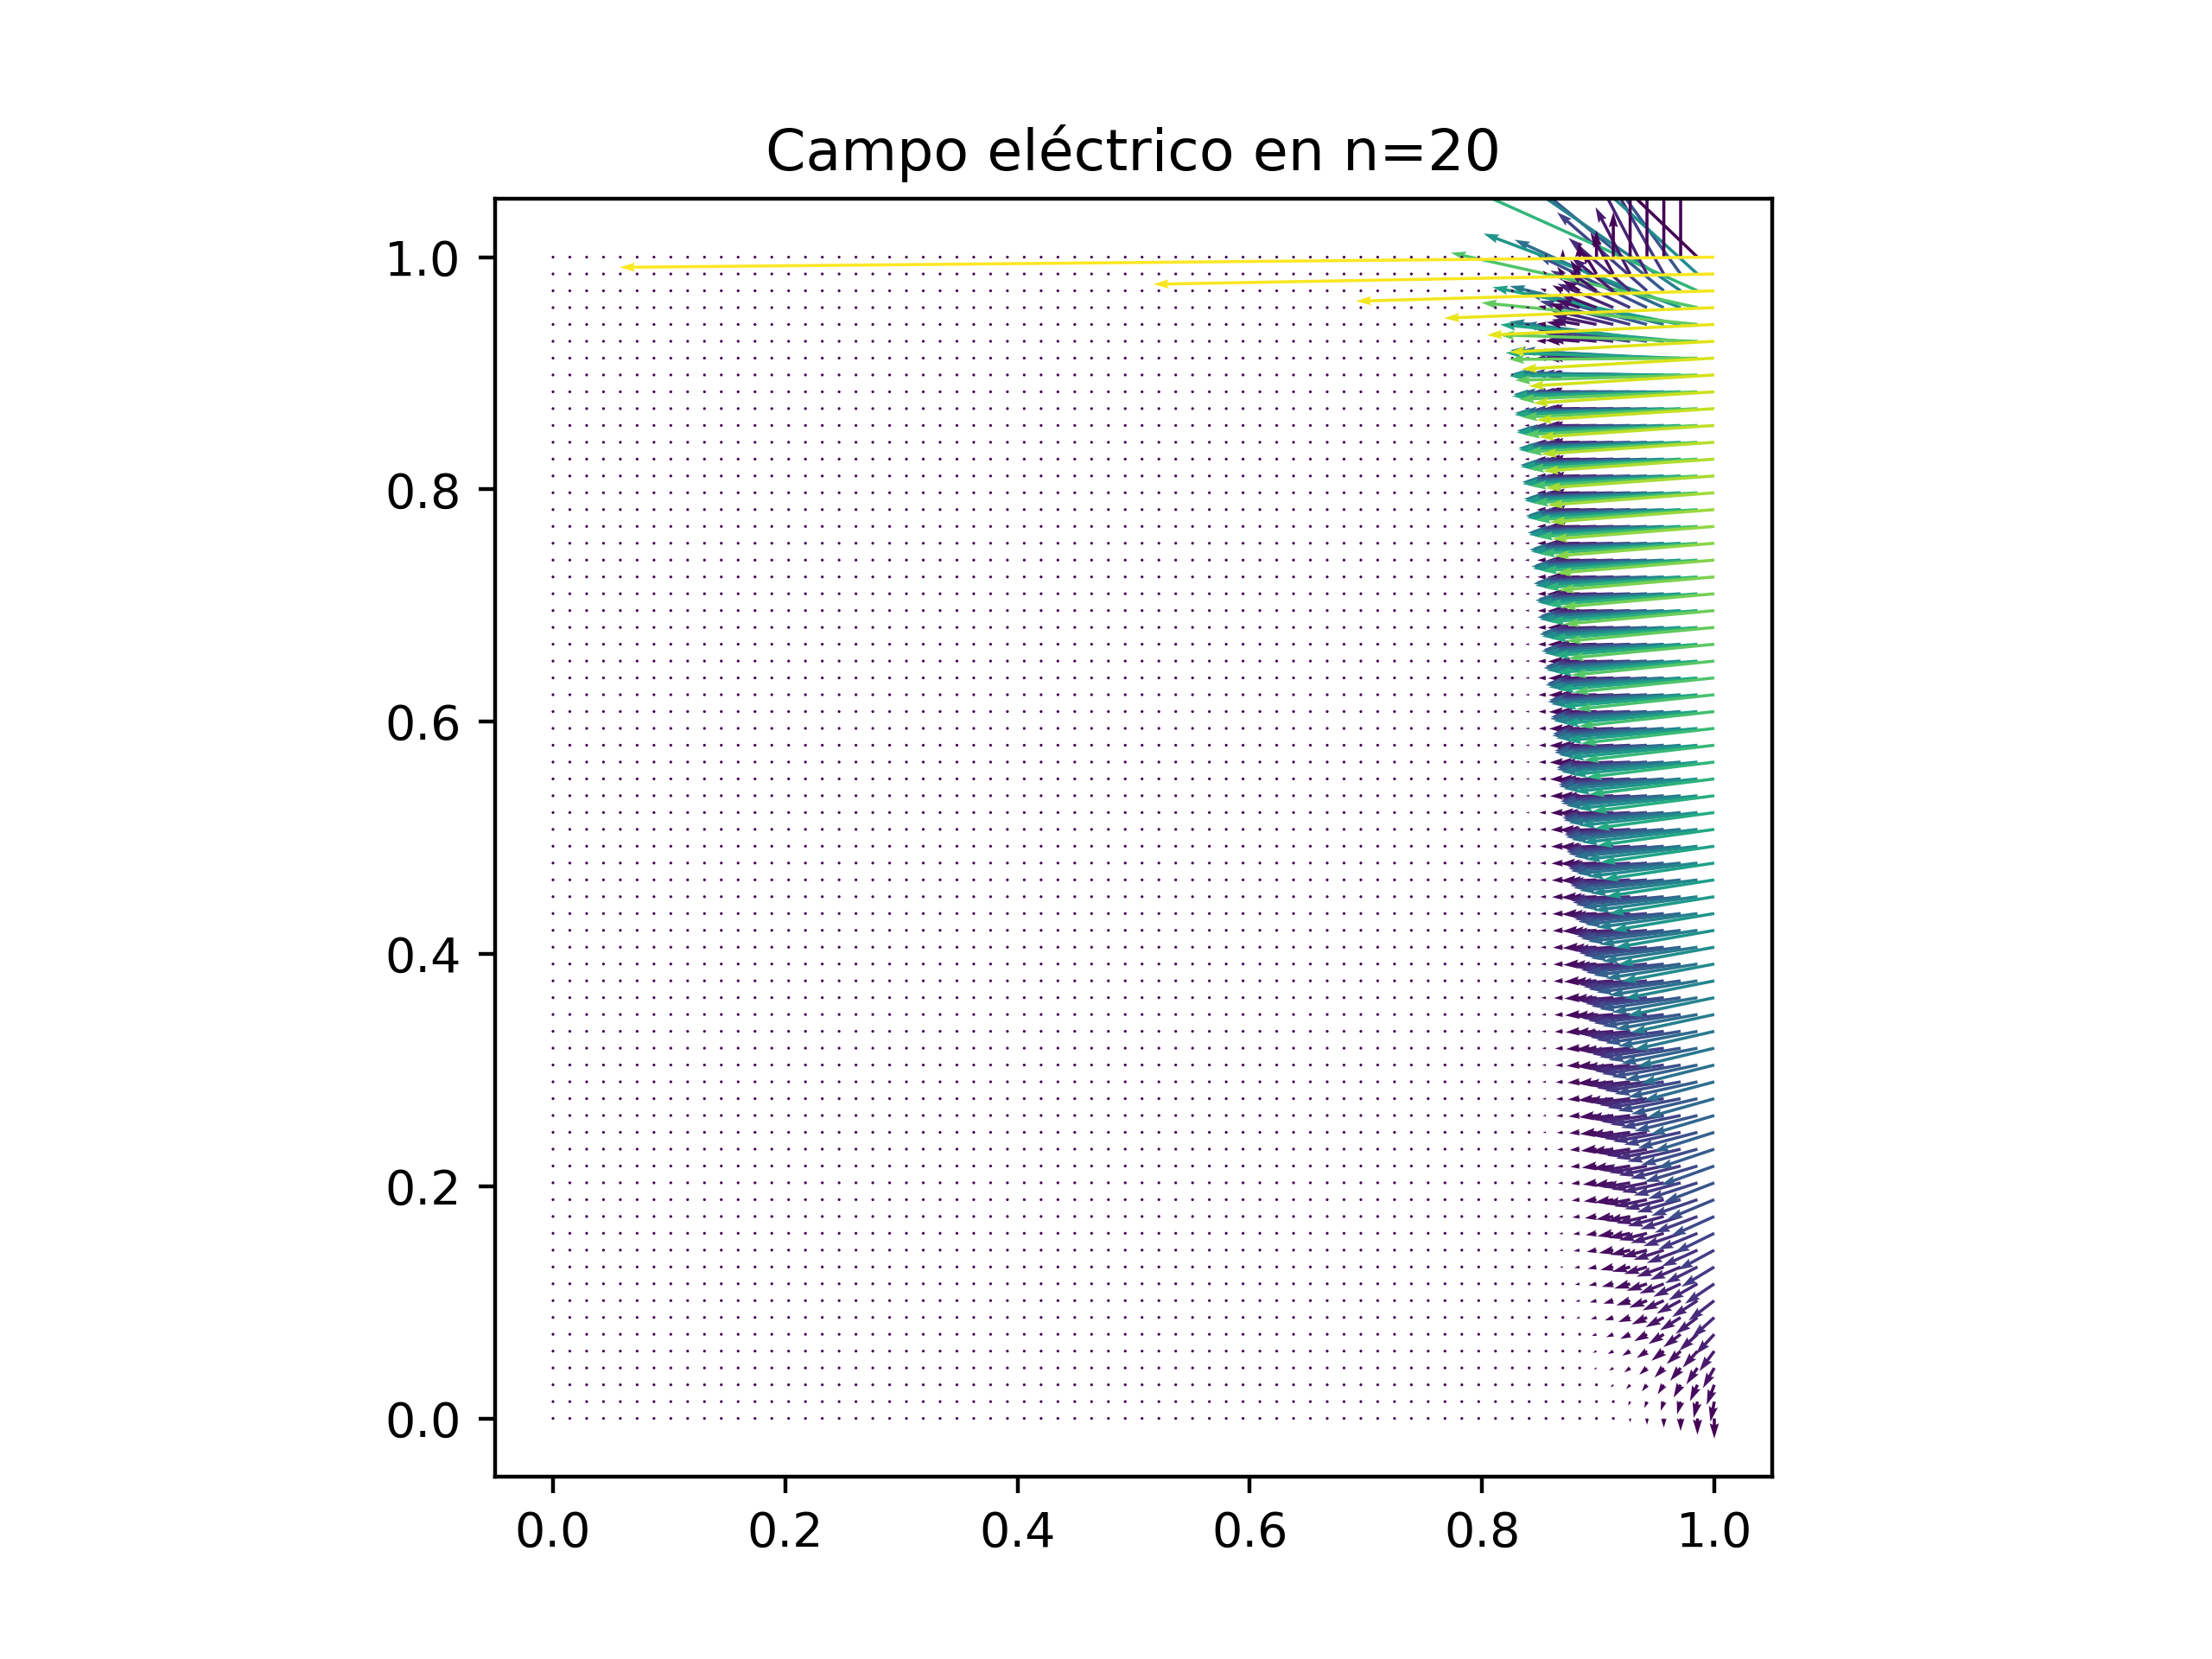
\includegraphics[width=2.8in]{images/arctan-field}
  \caption{Potencial y campo eléctrico para \(h(y) = tan^{-1}(y/a)\)}
  \label{arctan-n20}
\end{figure}

\begin{figure}
  \centering
  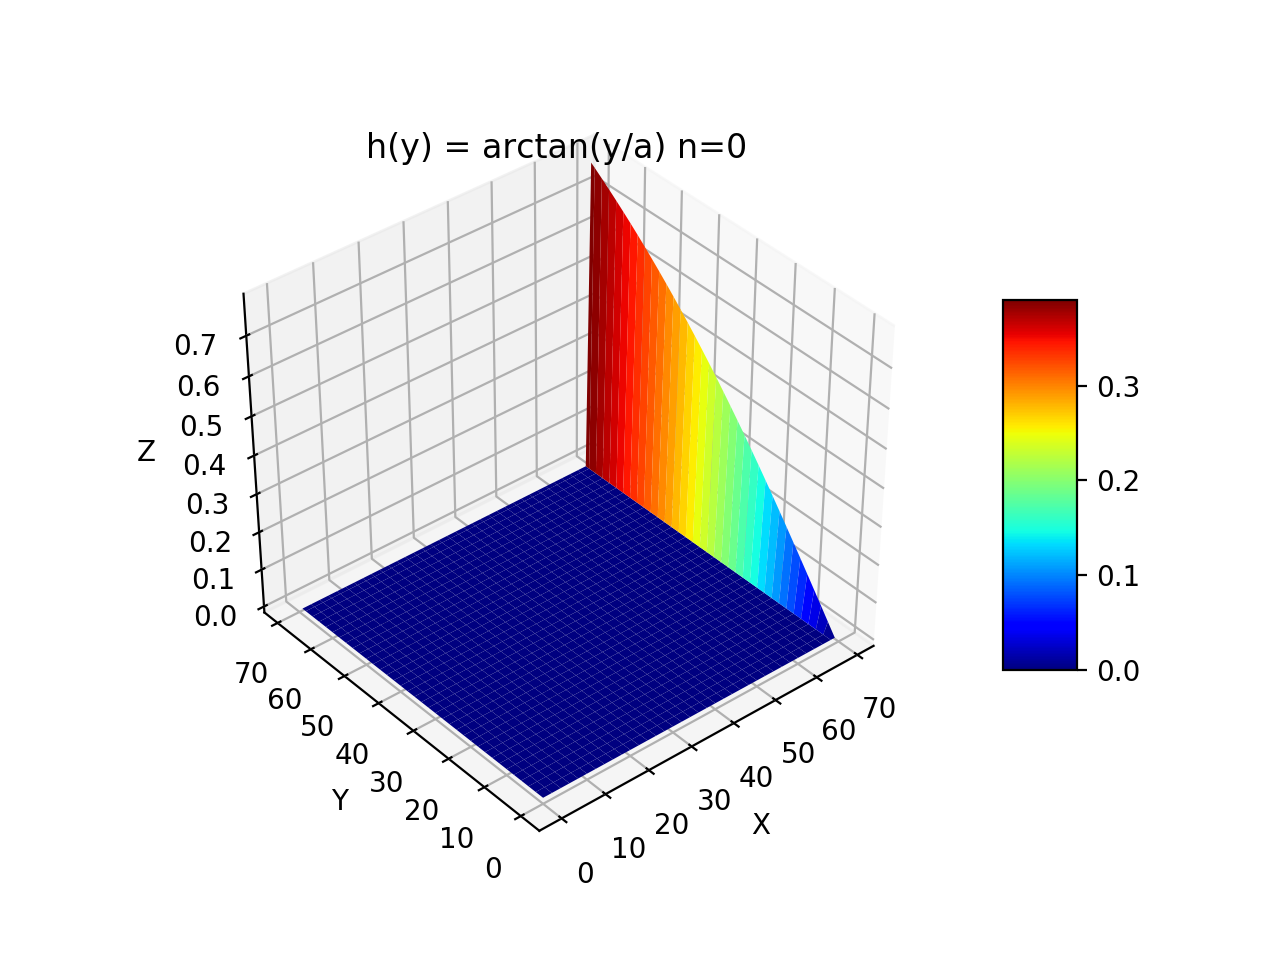
\includegraphics[width=1.5in]{images/arctan-n0}
  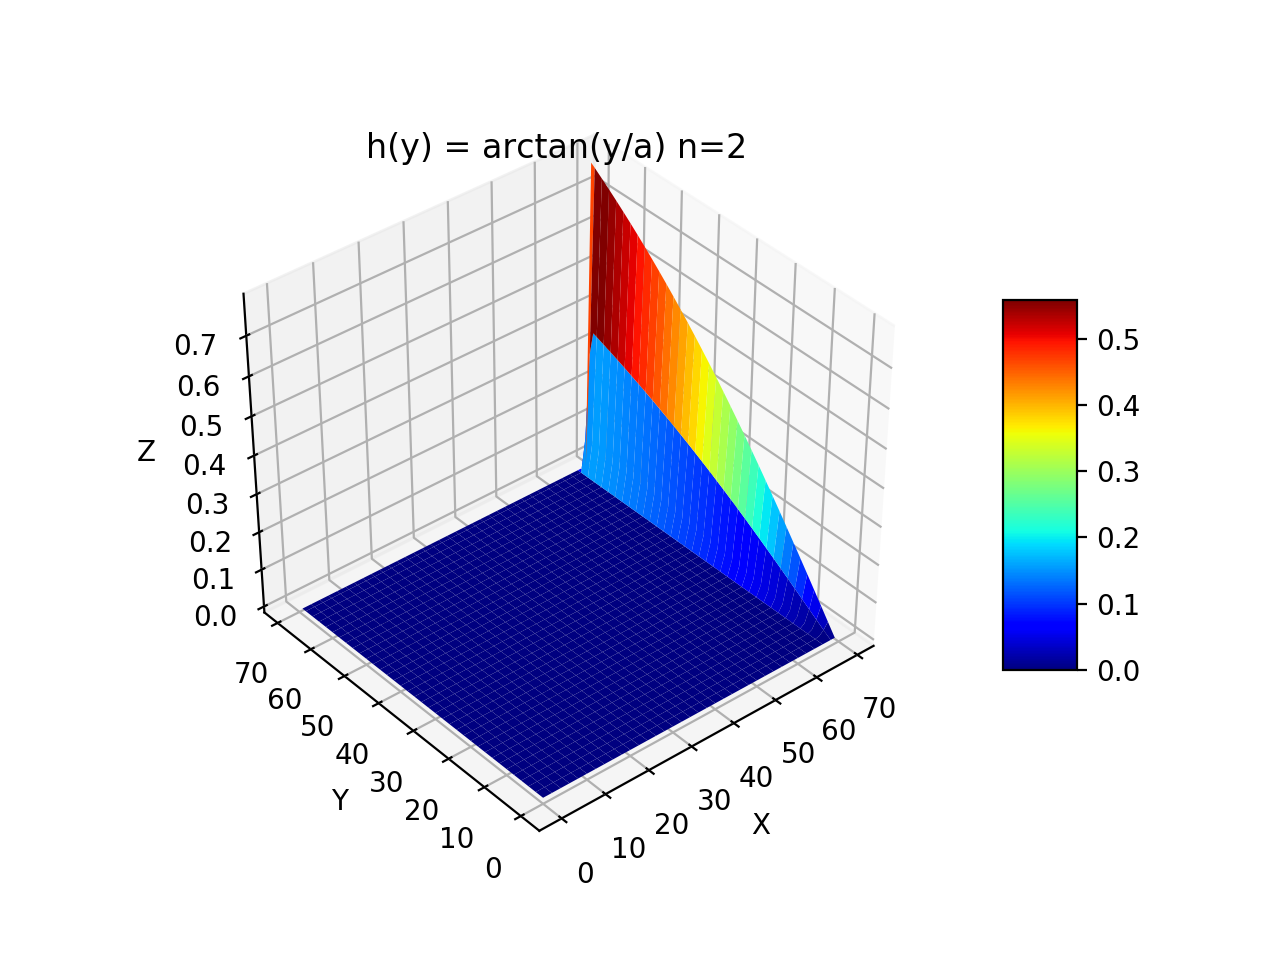
\includegraphics[width=1.5in]{images/arctan-n2}
  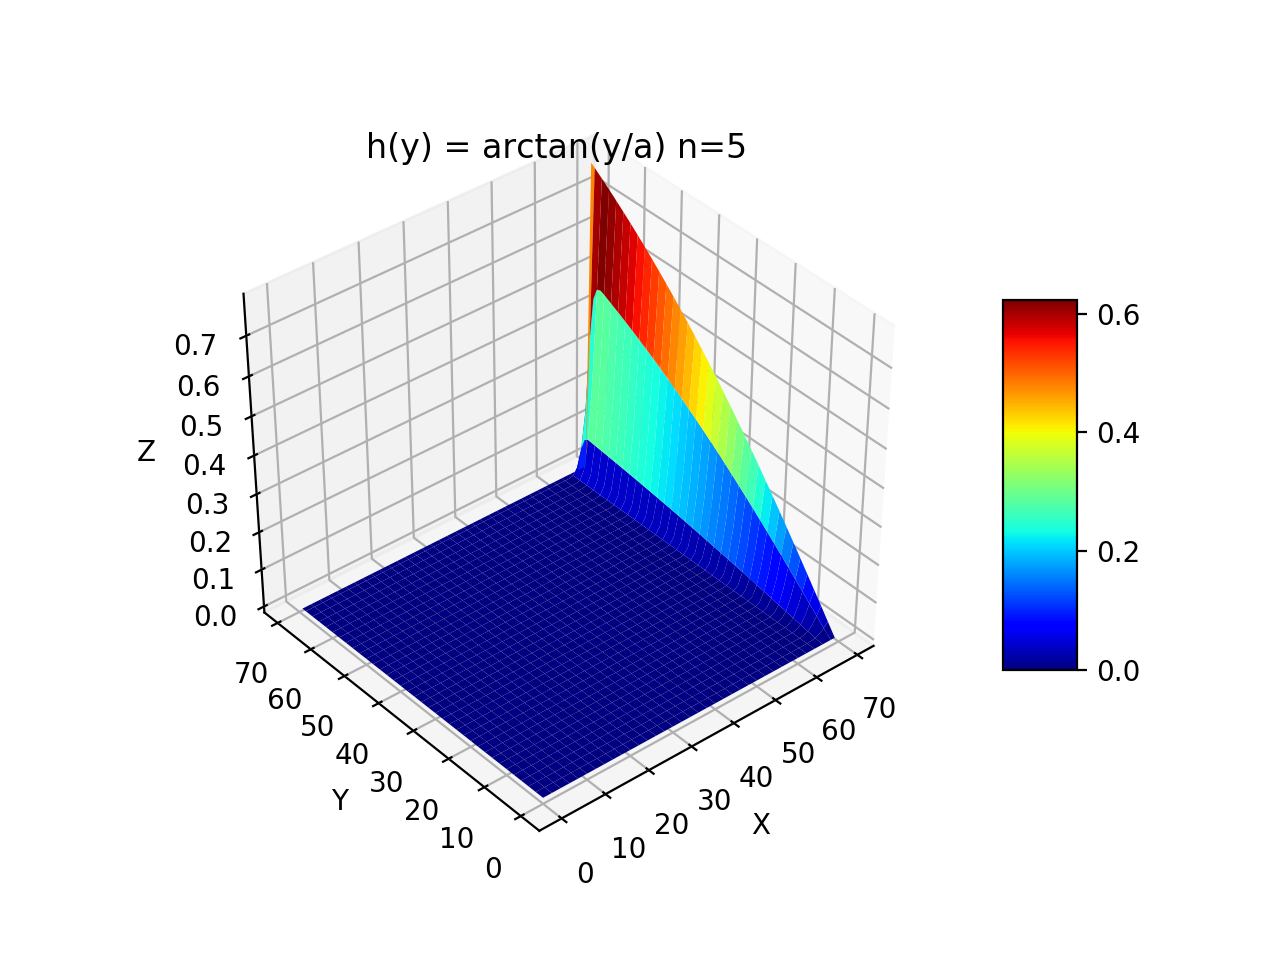
\includegraphics[width=1.5in]{images/arctan-n5}
  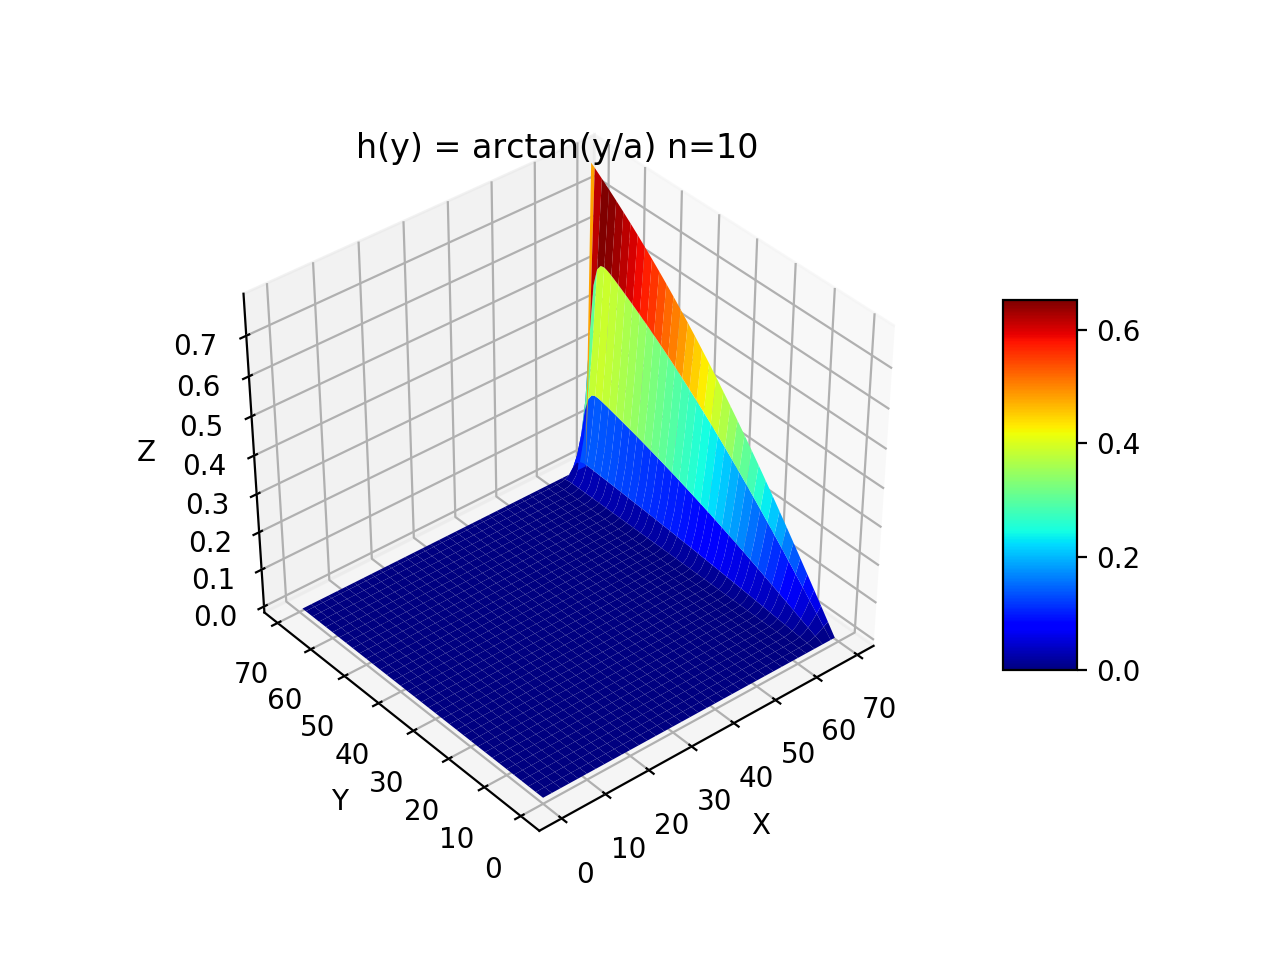
\includegraphics[width=1.5in]{images/arctan-n10}
  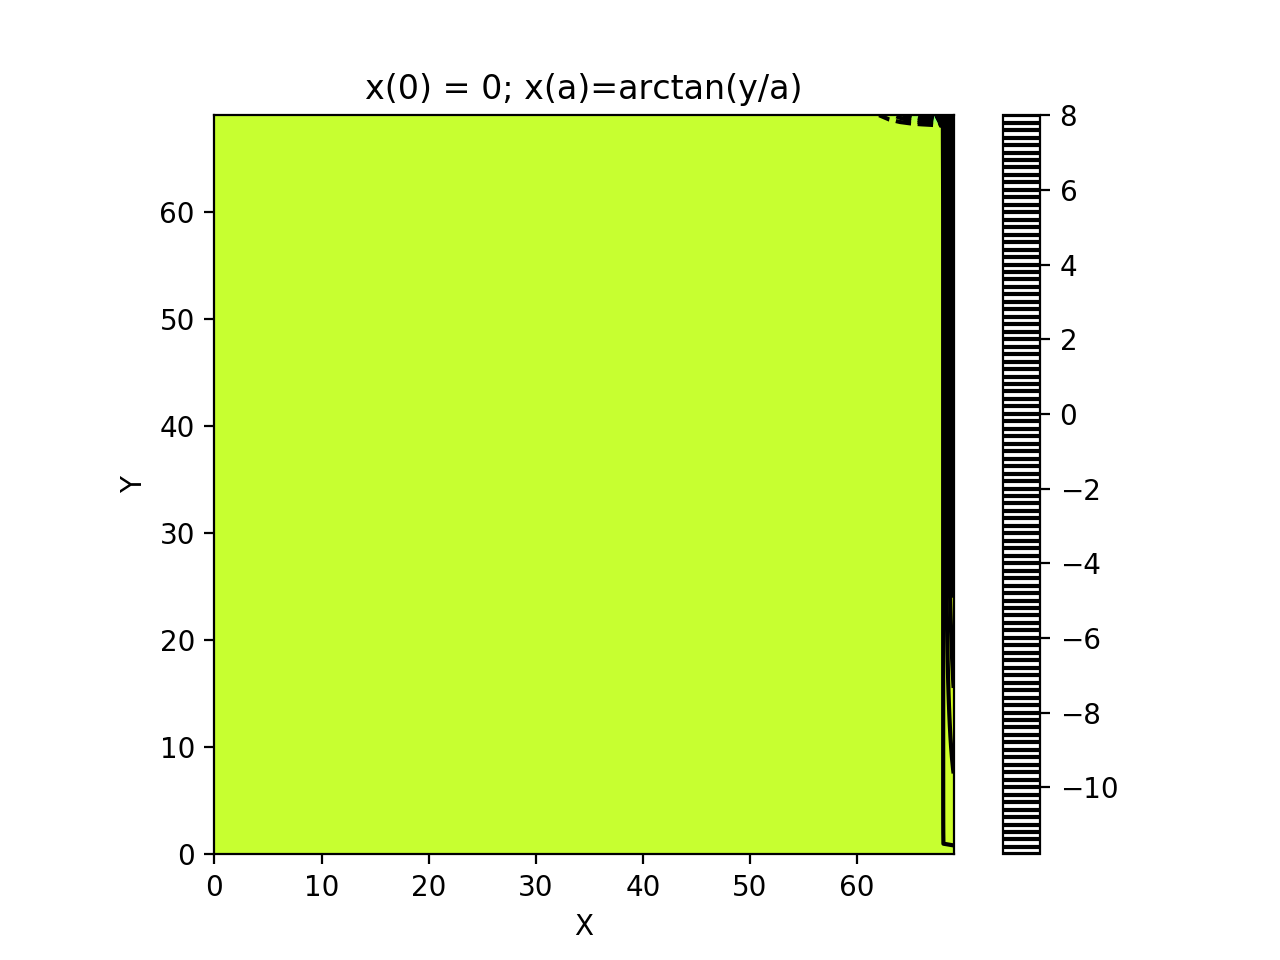
\includegraphics[width=1.5in]{images/arctan-density}
  \caption{\(h(y) = tan^{-1}(y/a)\) con iteraciones \(n = 0, 2, 5 \text{ y } 10\)}
  \label{arctan-iterations}
\end{figure}

Para este inciso se requiere resolver una forma alternativa en la que se elimina
el plano \(x=0\), para esta configuración se asumirá que el campo naturalmente tiene un
potencial de 0.1v para poder apreciar el efecto de los planos conectados a tierra.
\\\\
Como ya se incluye detalles de la solución anterior, solo mostraremos los graficos de \(n=20\).

\begin{figure}
  \centering
  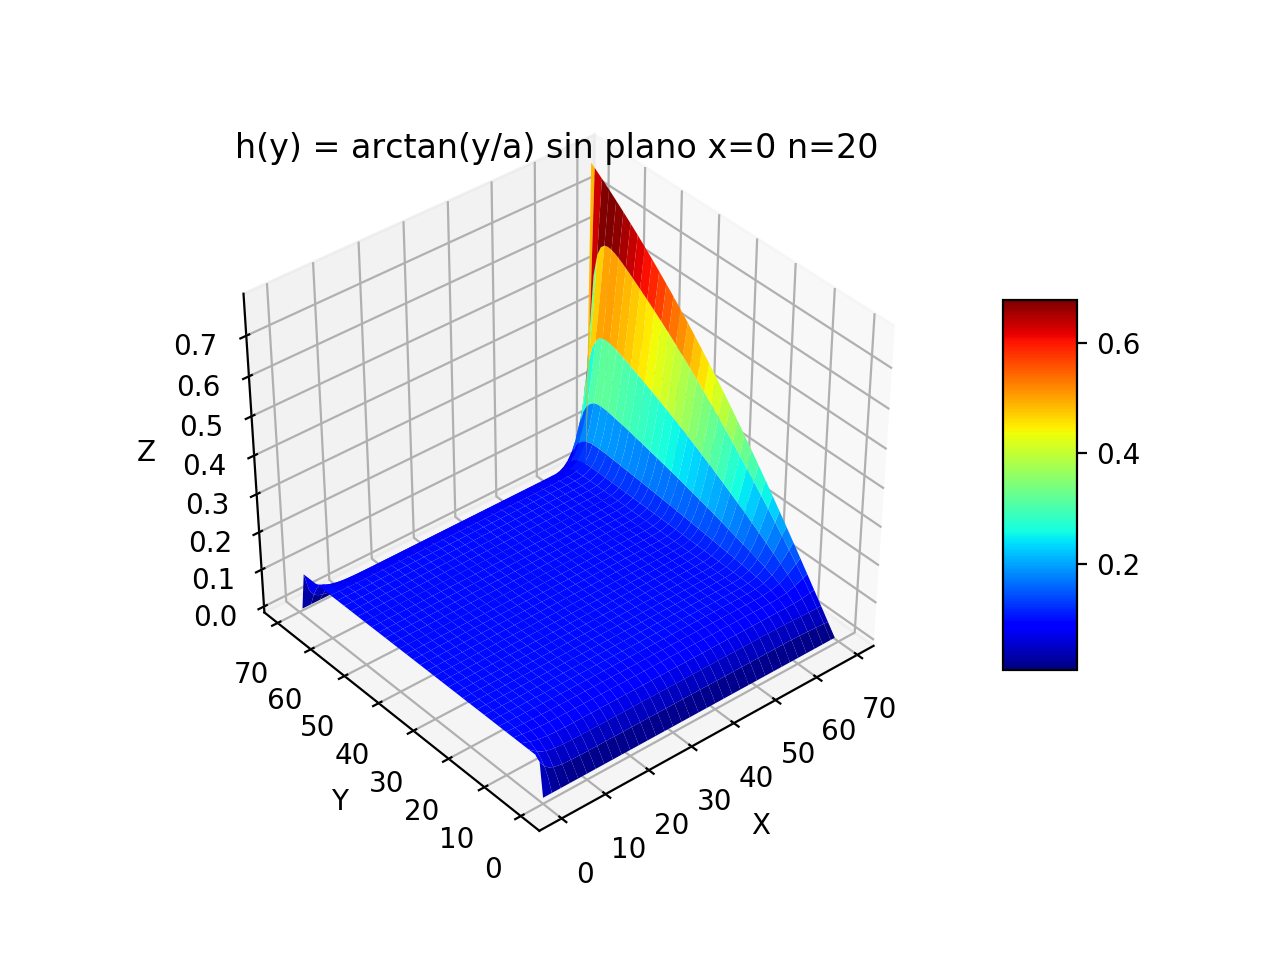
\includegraphics[width=2.8in]{images/arctan-alt-n20}
  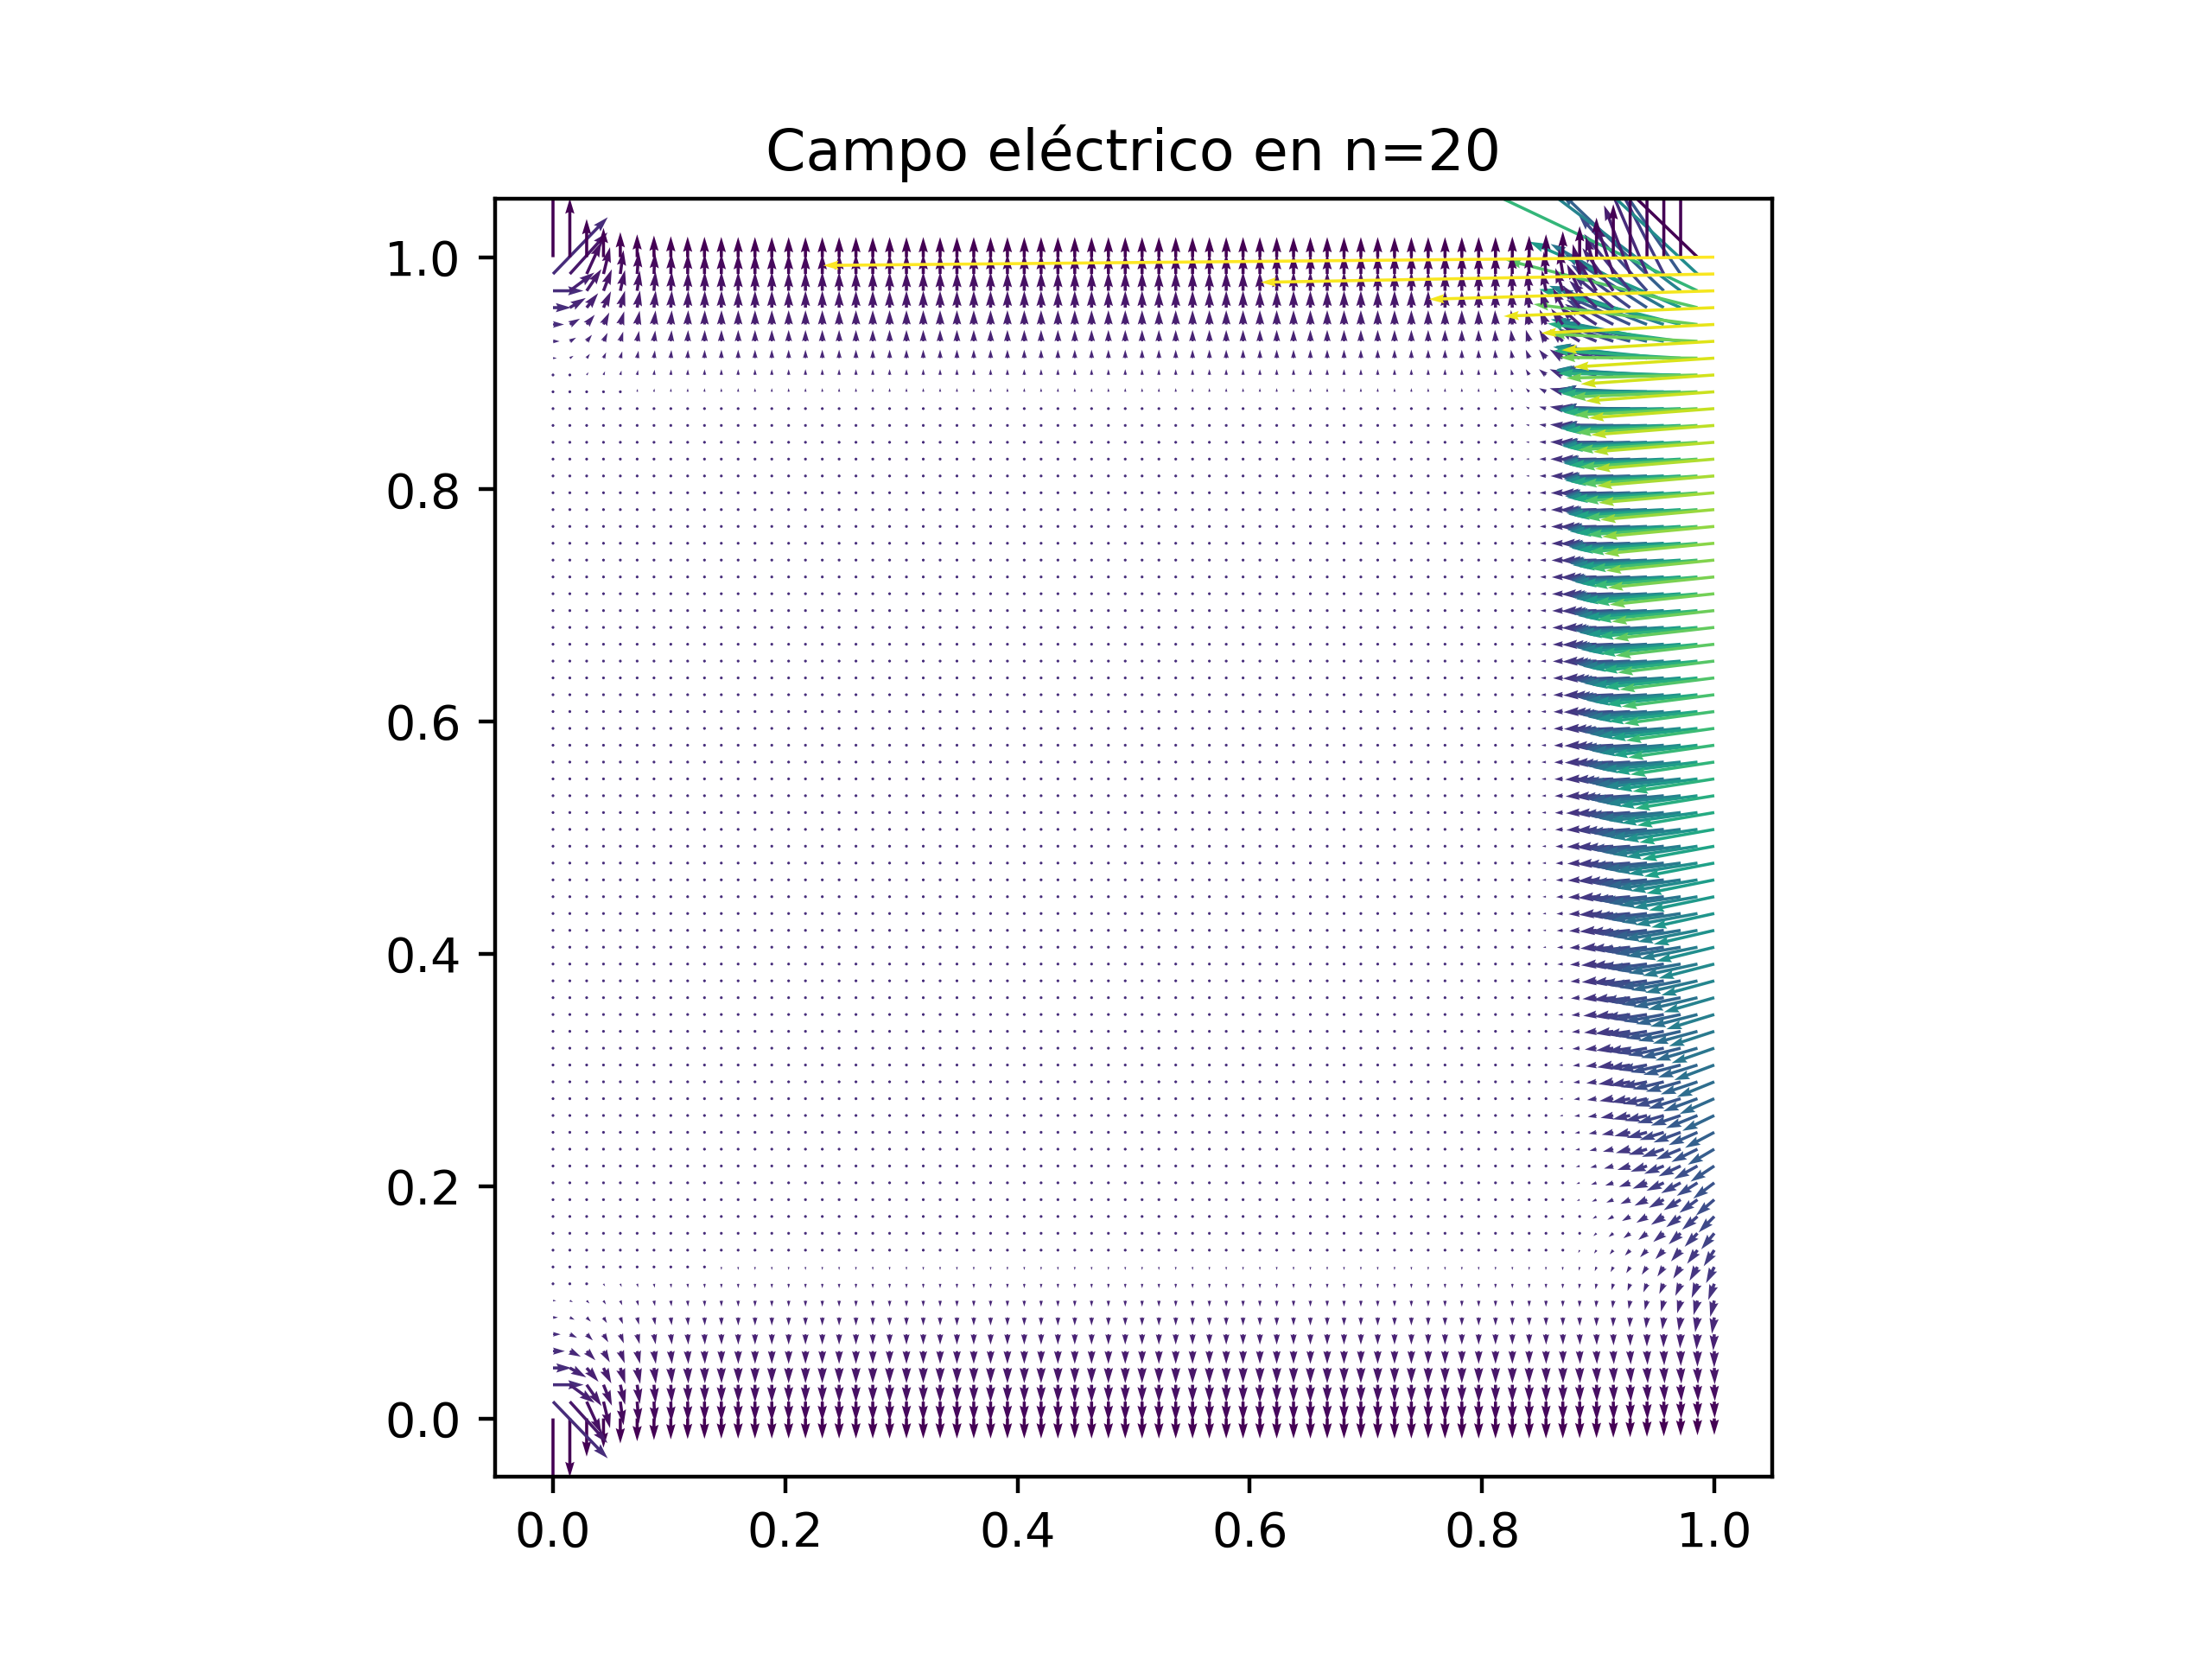
\includegraphics[width=2.8in]{images/arctan-alt-field}
  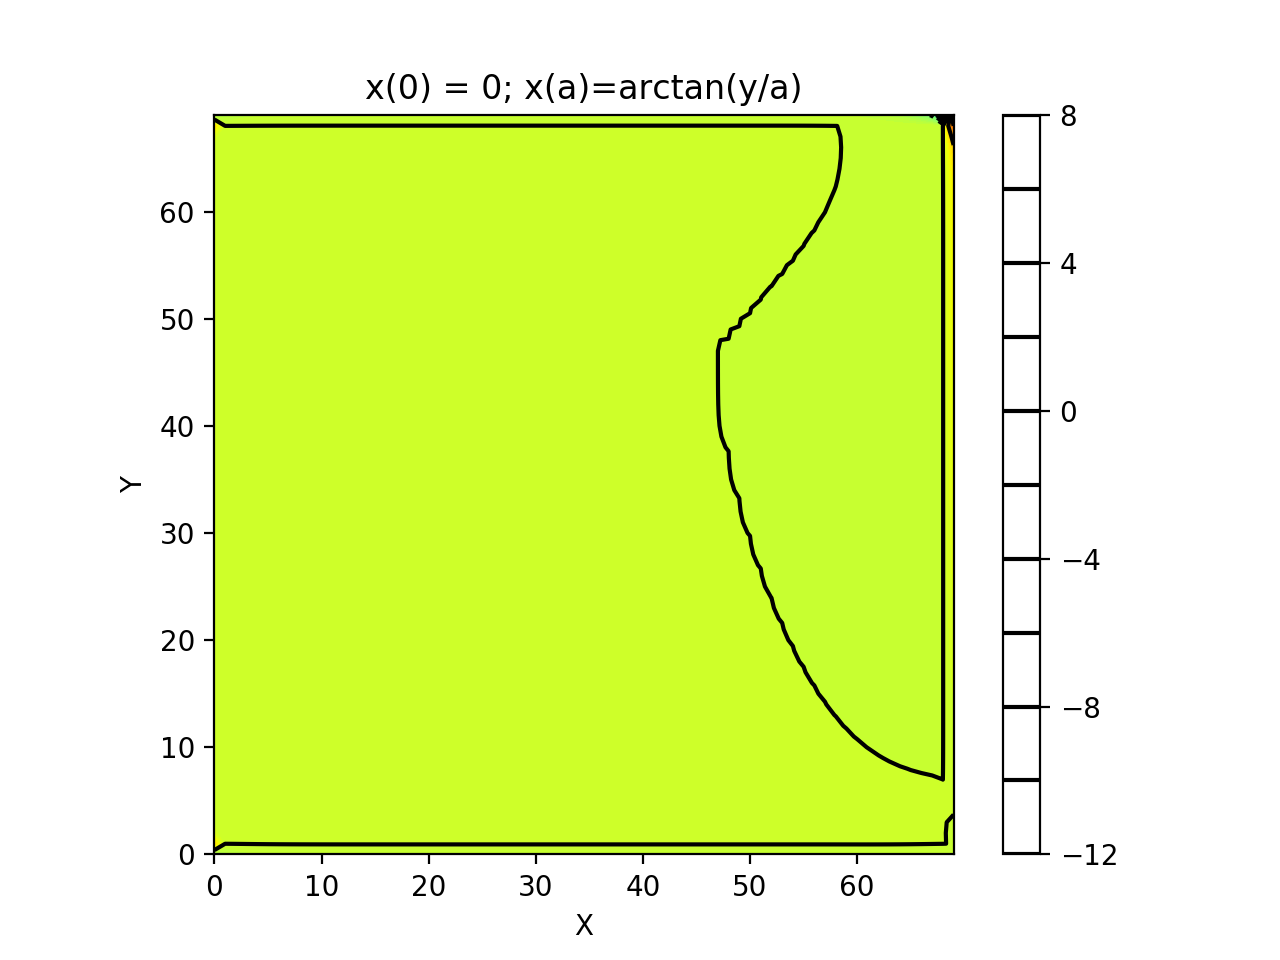
\includegraphics[width=1.5in]{images/arctan-alt-density}
  \caption{Potencial, campo eléctrico para \(h(y) = tan^{-1}(y/a) sin x=0\)}
  \label{arctan-n20}
\end{figure}


\pagebreak

\subsubsection{Cambio de condiciones}

Si el plano \(x=0\) se corre a \(x=-b\), y se tiene
\\
\(g(y)=h(y)=2y^3+5\) 
\\\\
Para este inciso se necesitan dos condiciones de frontera distintas de cero y valores en el plano negativo.
Gracias a que función de condicion de frontera es independiente de \(x\) simplemente duplicaremos el tamaño del
espacio en ese eje, es decir las condiciones iniciales se presentarán en \(x=0, x=2b\).
En el código las configuramos de esta forma

\begin{lstlisting}
  T[:,-1] = 2*y**3+5
  T[:,0] = 2*y**3+5
\end{lstlisting}

Así como el ejercicio anterior, presentamos el mapa de calor y el campo eléctrico de la iteración \(n=20\) en la figura \ref{2y3-n20} seguido de 
las iteraciones menores, densidad y condiciones iniciales (figura \ref{2y3-iterations}).

\begin{figure}
  \centering
  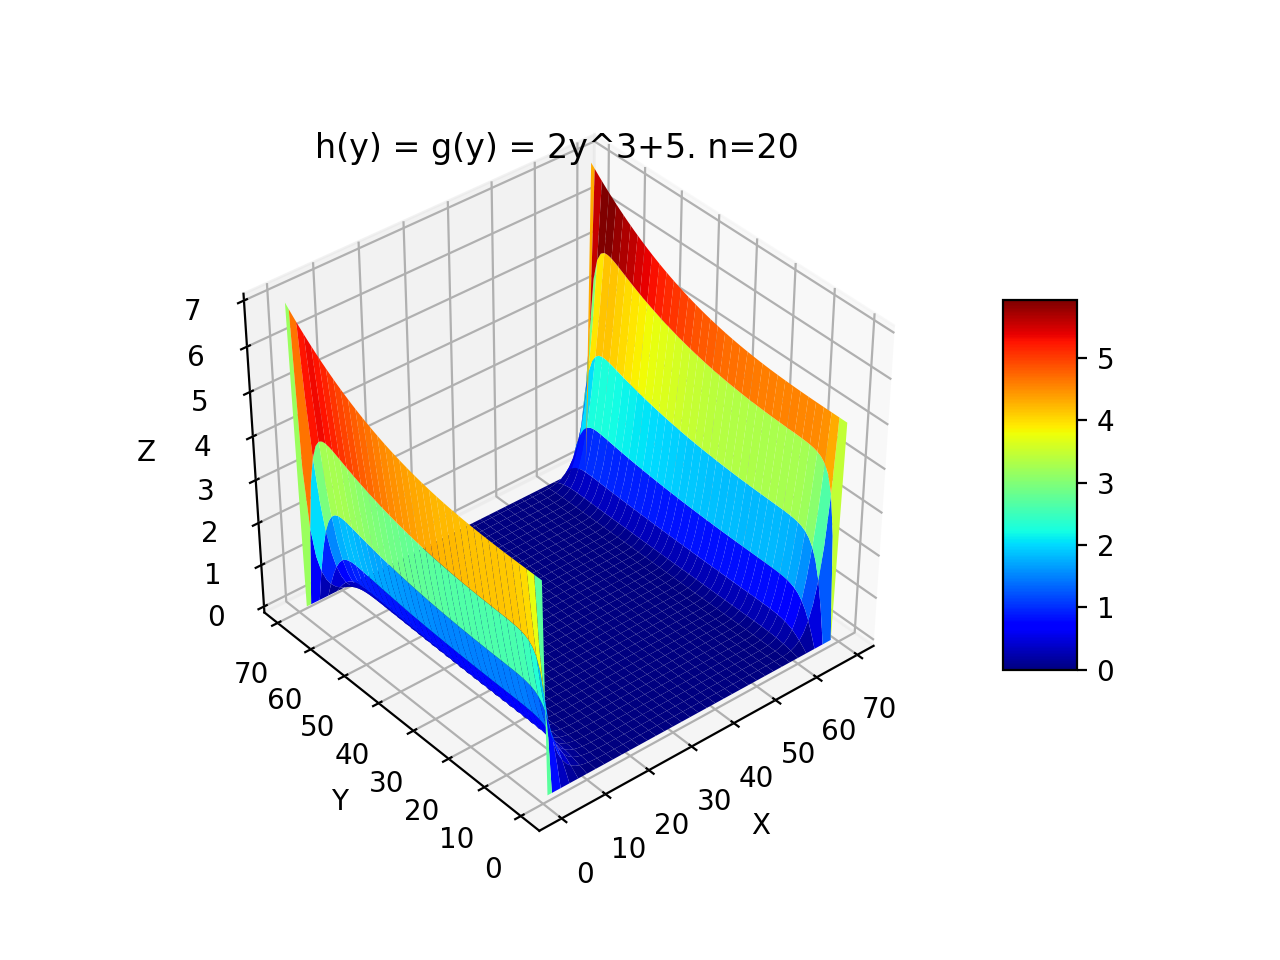
\includegraphics[width=2.8in]{images/2y3-n20}
  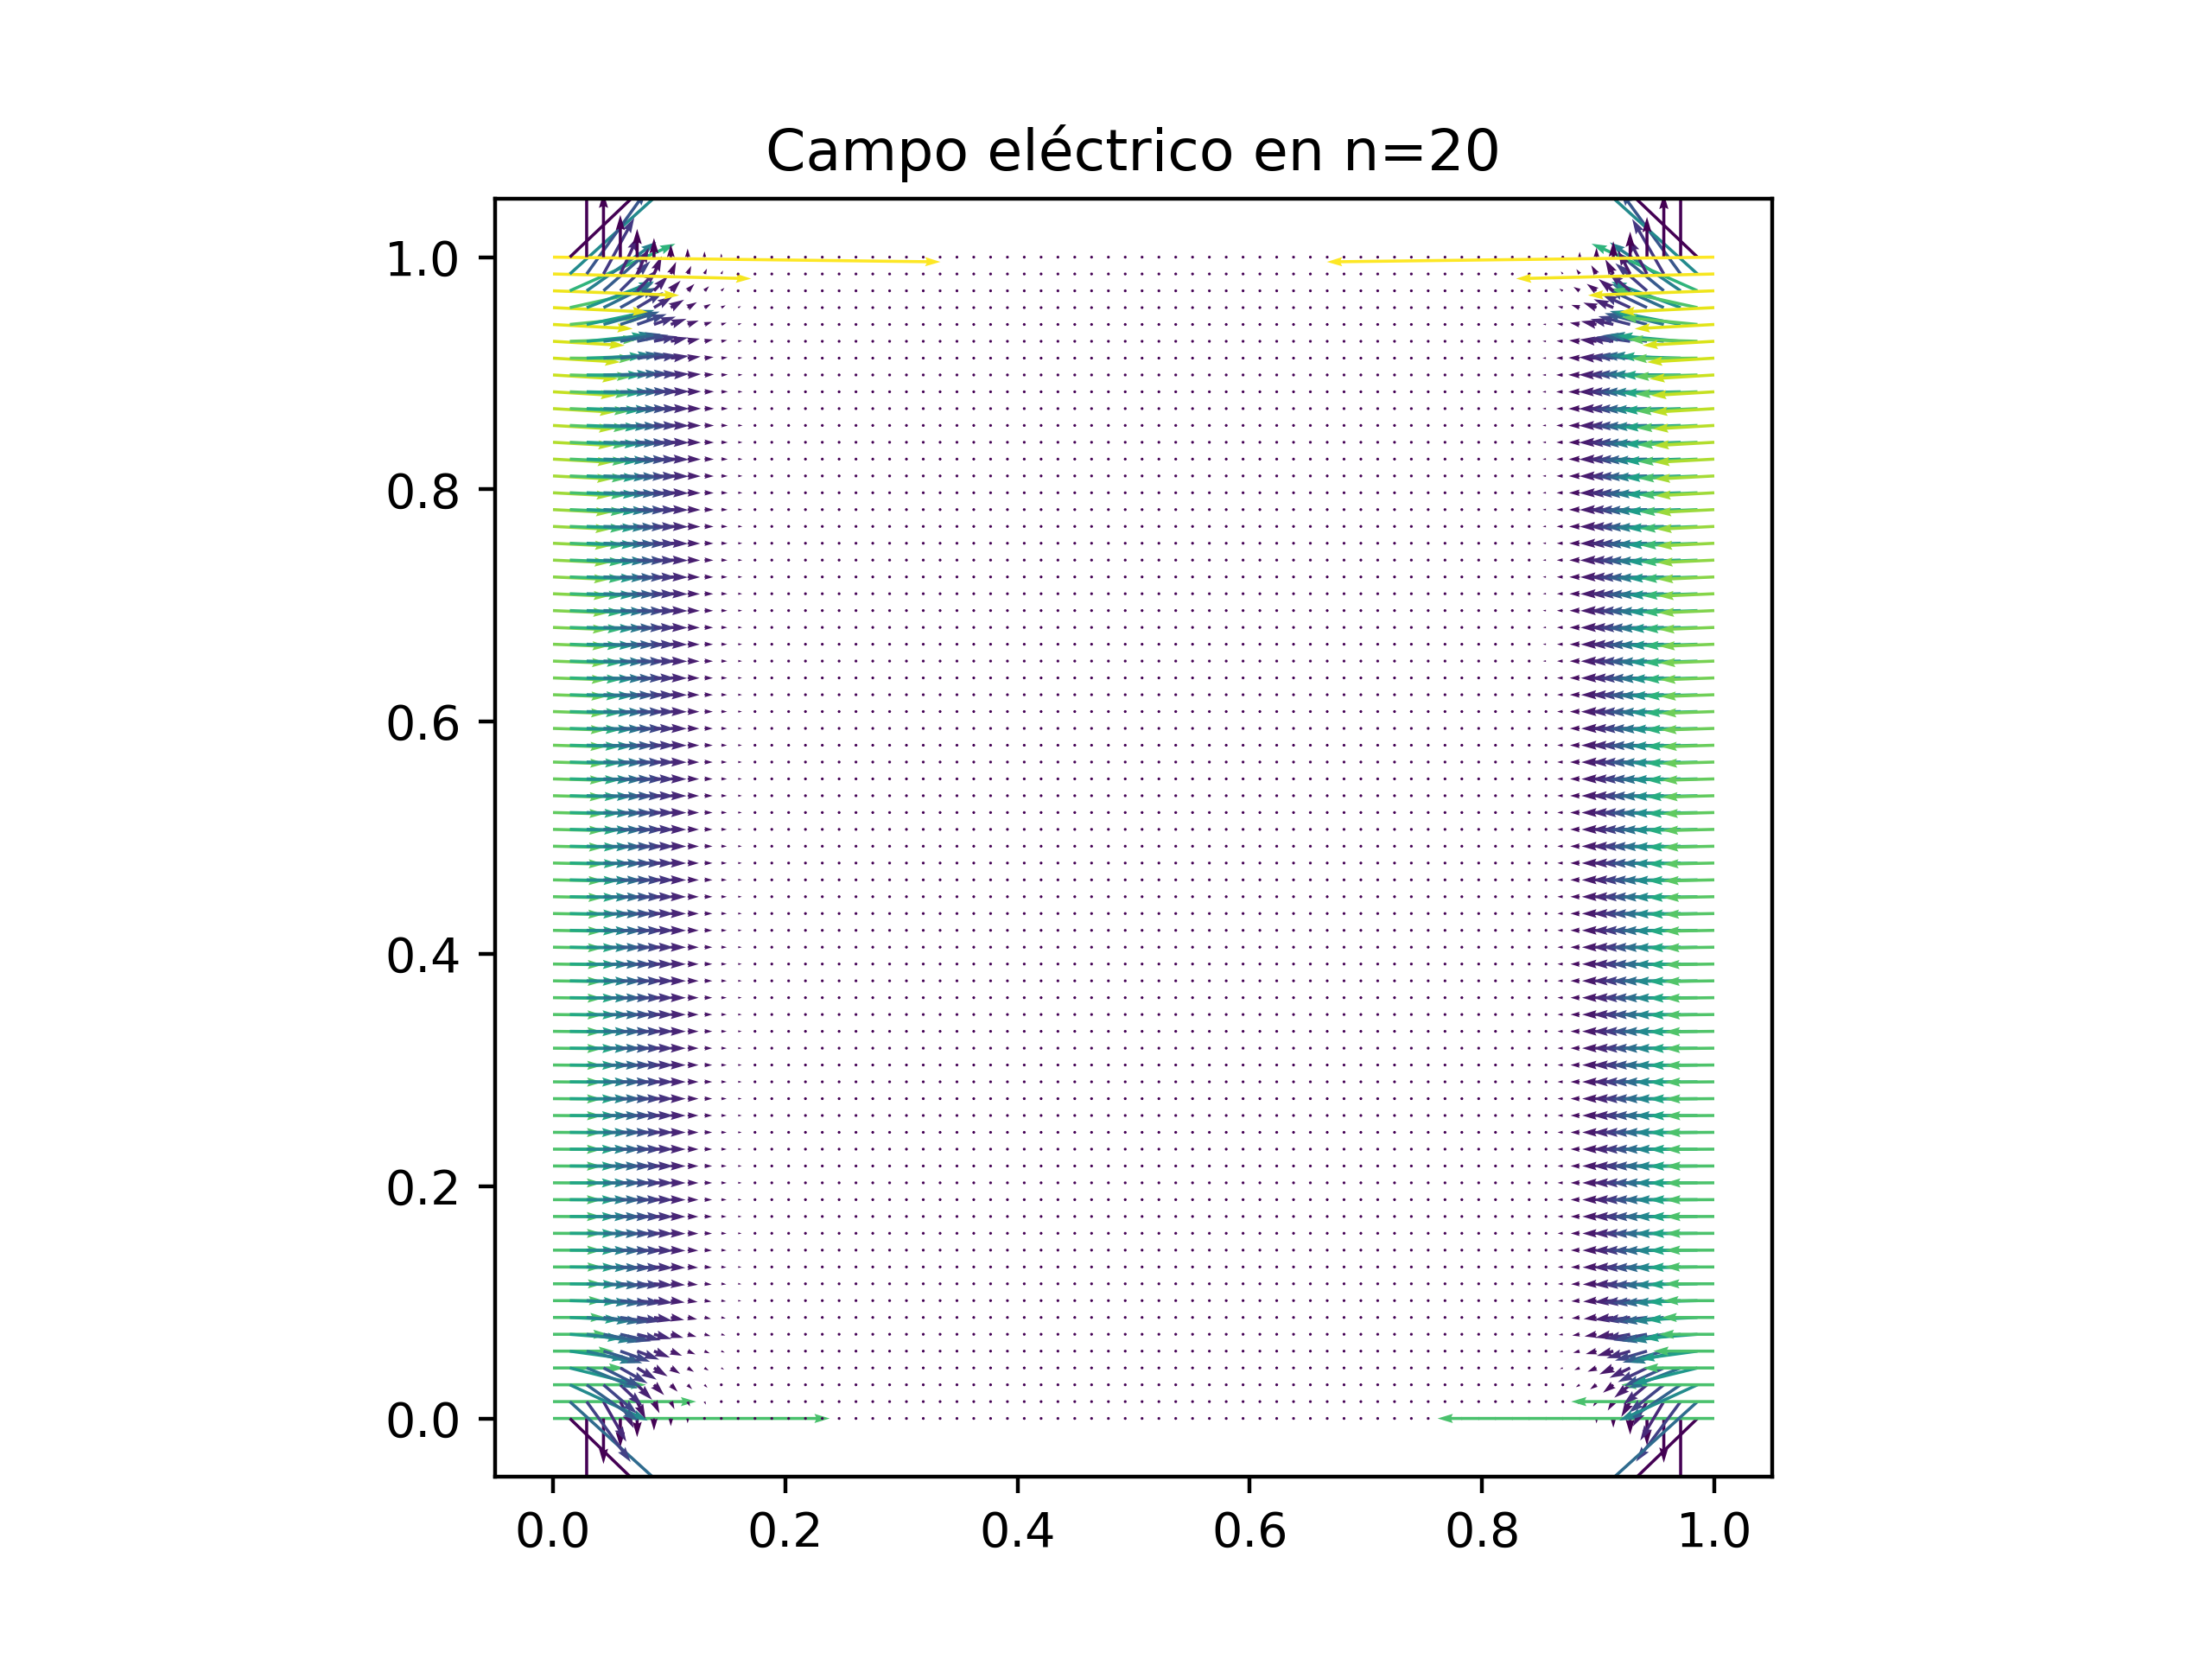
\includegraphics[width=2.8in]{images/2y3-field}
  \caption{Potencial y campo eléctrico para \(h(y) = g(y) = 2y^3+5\)}
  \label{2y3-n20}
\end{figure}

\begin{figure}
  \centering
  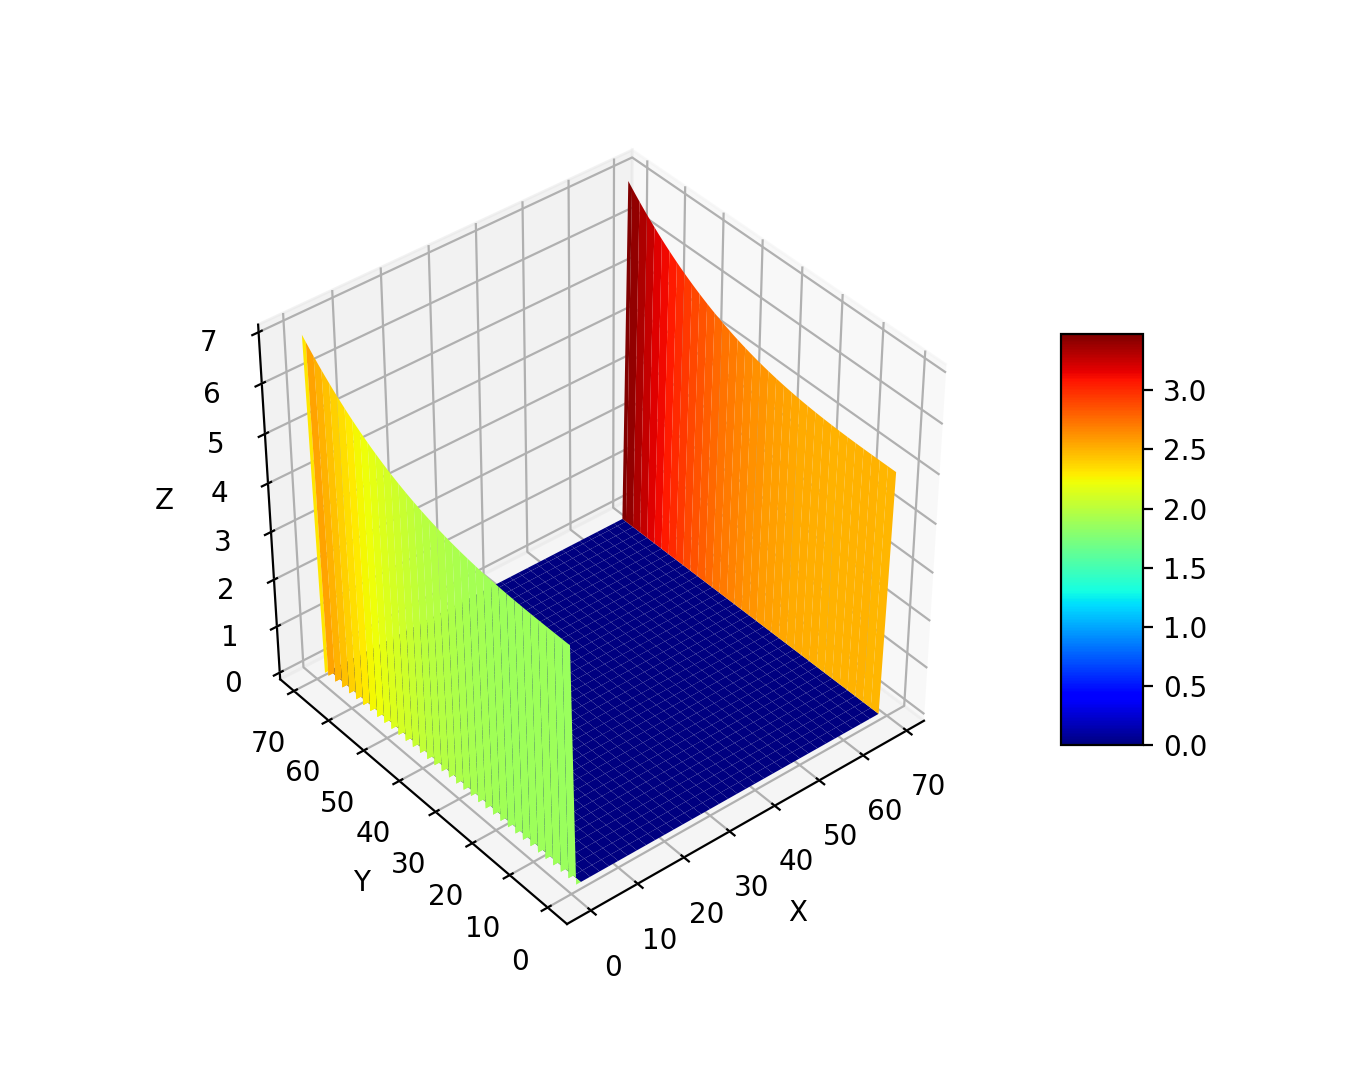
\includegraphics[width=1.5in]{images/2y3-n0}
  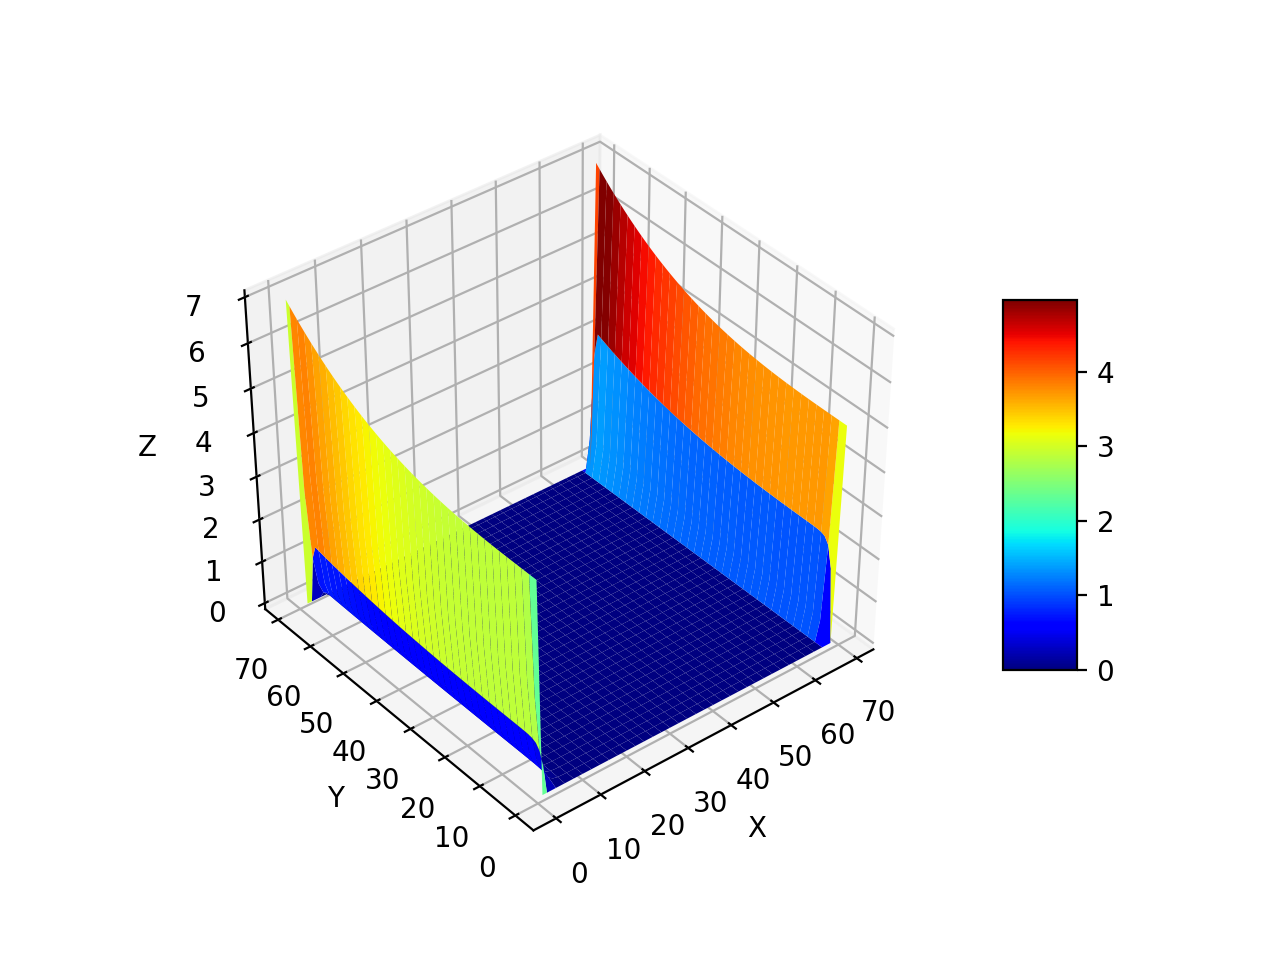
\includegraphics[width=1.5in]{images/2y3-n2}
  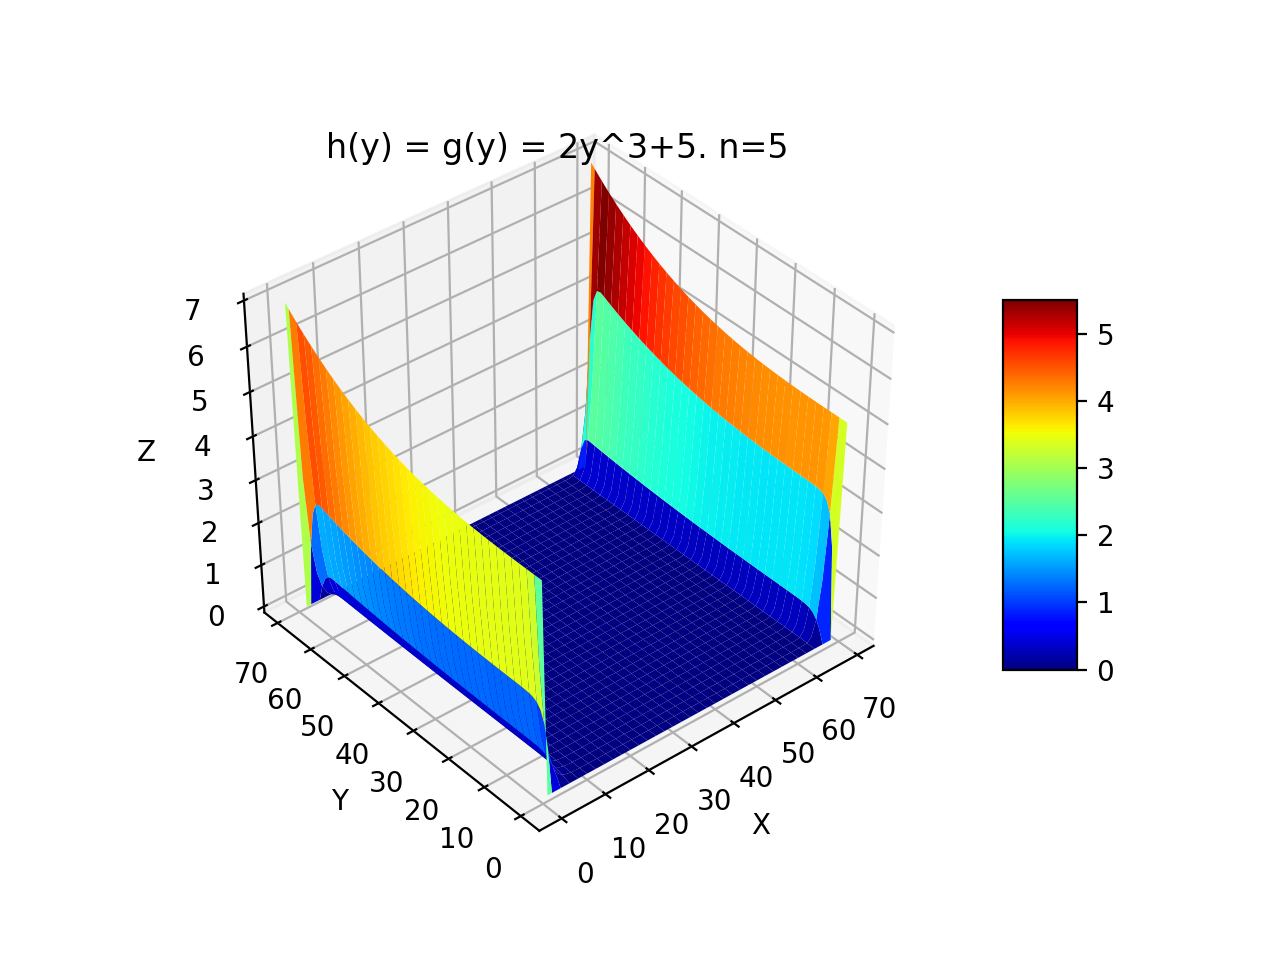
\includegraphics[width=1.5in]{images/2y3-n5}
  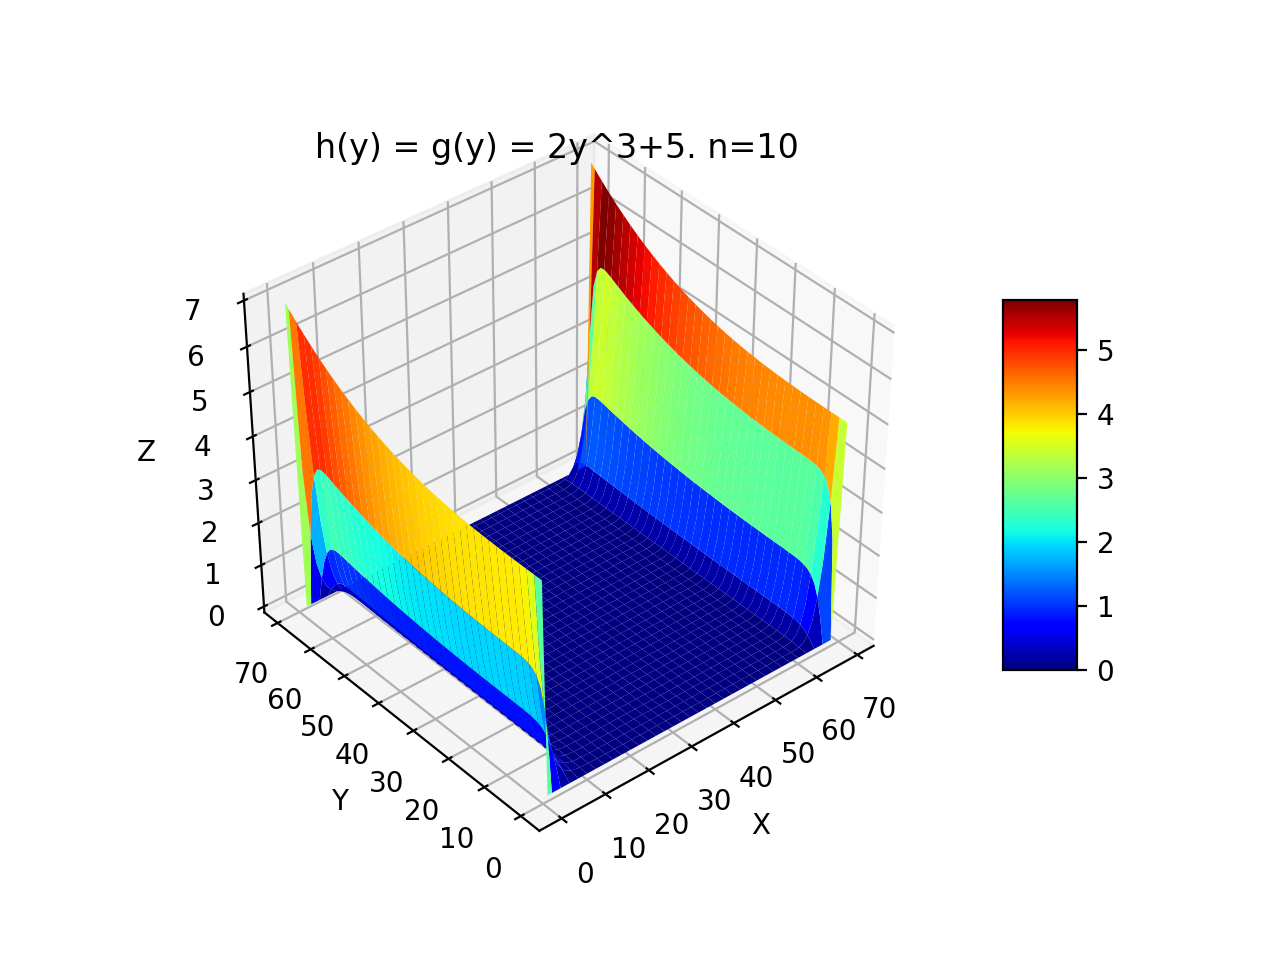
\includegraphics[width=1.5in]{images/2y3-n10}
  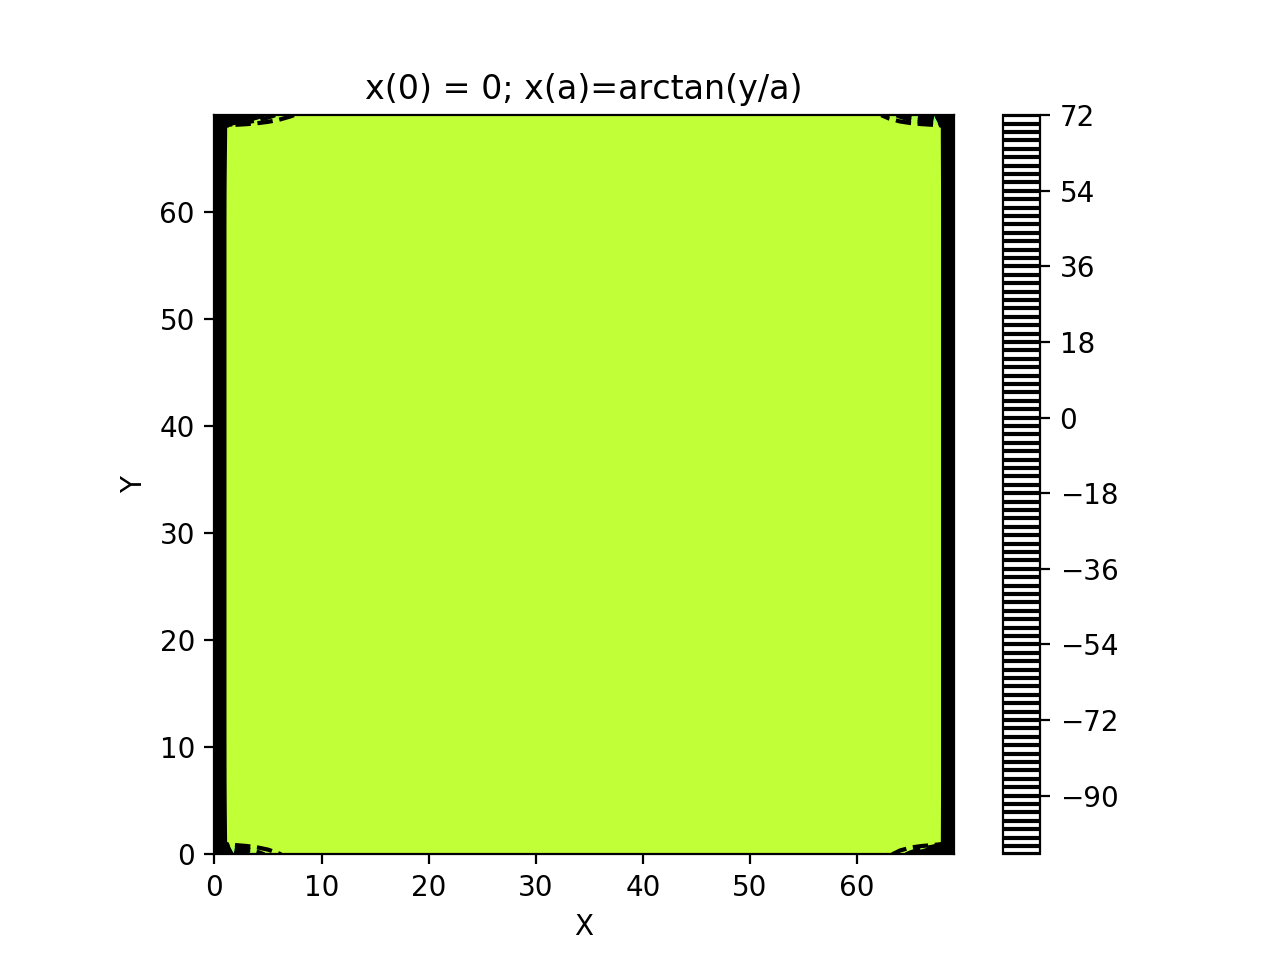
\includegraphics[width=1.5in]{images/2y3-density}
  \caption{\(h(y) = g(y) = 2y^3+5\) con iteraciones \(n = 0, 2, 5 \text{ y } 10\)}
  \label{2y3-iterations}
\end{figure}

/subsubsection{Problema de Laplace en 3D}

Una tubería se extiende a lo largo del eje z
y posee paredes en \(x = y = z=0,x=a y=b\). La placa en \(z=0\) se encuentra a potencial
\(f(x,y) = xy^2\), y las demás están aterrizadas.
Elija valores de a y b de tal manera que las gráficas puedan apreciarse correctamente.
Realice las gráficas para \(n= 2, 5, 10, 20\)

Para poder graficar correctamente este ejercicio, utilizaremos la misma función de antes para
generar mapas de calor en 3D, pero en este caso agregaremos distintos nuevos para valores de z.

Utilizando matplotlib, es facil agregar planos utilizando:

\begin{lstlisting}
  # agregamos alpha para poder ver todos los planos
  ax.plot_surface(x,y,field[z]+z, alpha=0.3)
\end{lstlisting}

El otro cambio que debemos hacer es adaptar la función de relajación para funcionar en un campo 3D.
Basta con agregar:
\begin{lstlisting}
  # La funcion se queda igual excepto por agregar terminos de K
  field[i, j, k] = 1/6 * (field[i+1][j][k] ... field[i][j][k+1] + field[i][j][k-1])
\end{lstlisting}

Finalmente iteramos la nueva función con los arreglos y obtenemos un excelente resultado mostrado en 
figura \ref{xy2-n20}, como siempre, las iteraciones menores a menor detalle en \ref{xy2-iterations}

\begin{figure}
  \centering
  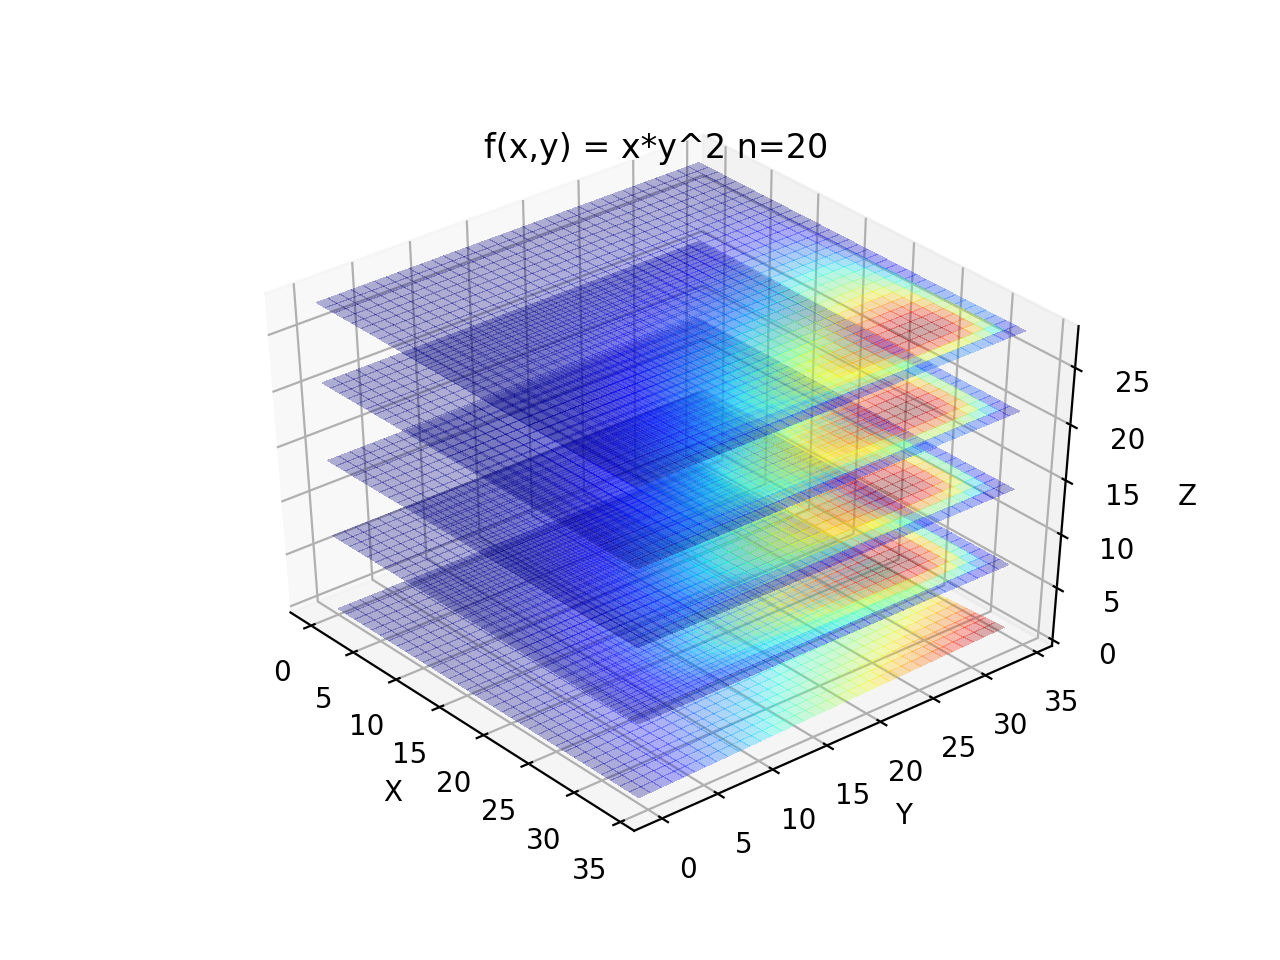
\includegraphics[width=2.8in]{images/xy2-n20}
  \caption{Potencial y campo eléctrico para \(f(x,y) = xy^2\)}
  \label{xy2-n20}
\end{figure}

\begin{figure}
  \centering
  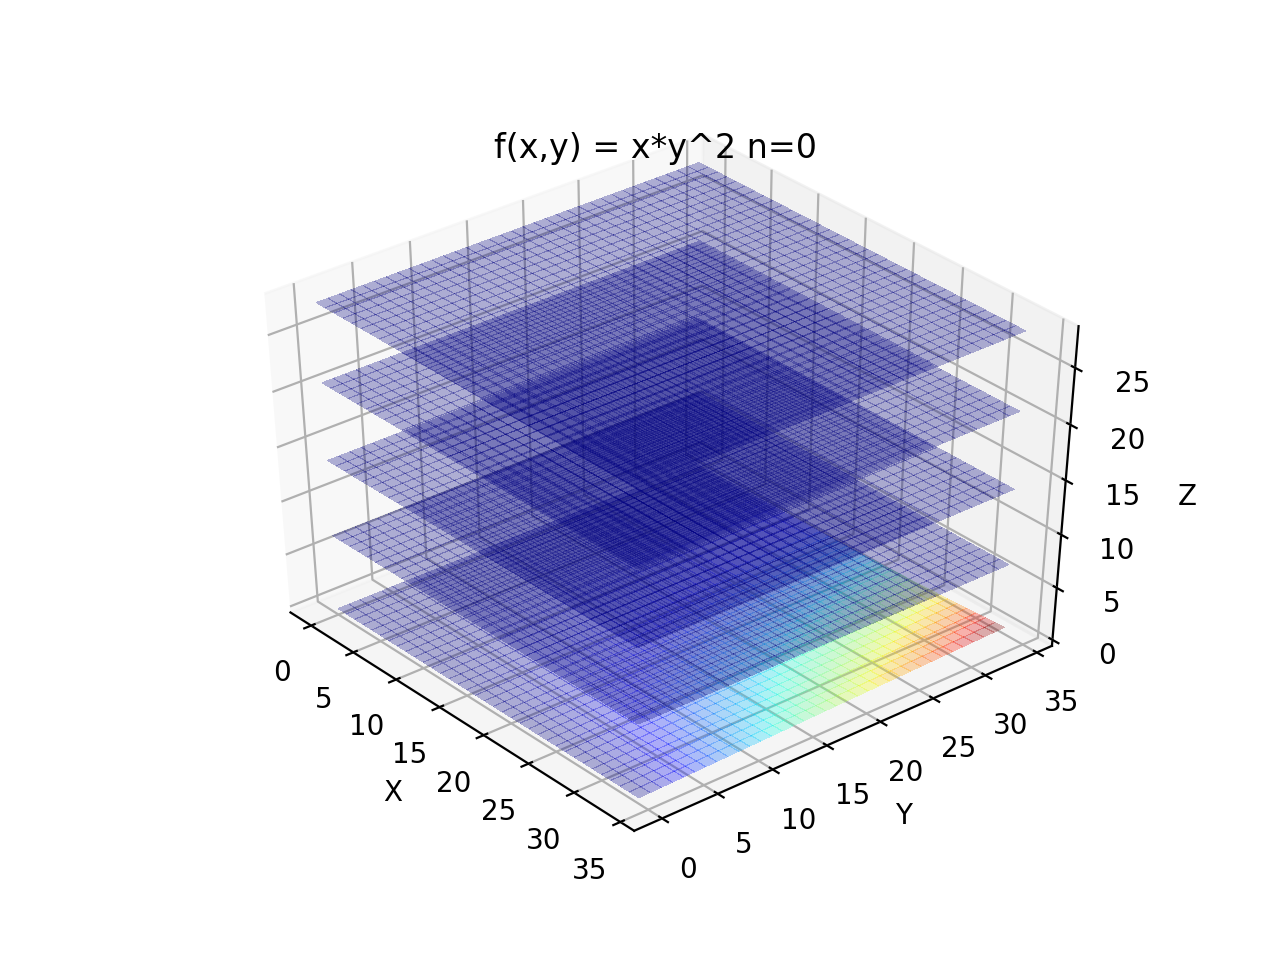
\includegraphics[width=1.5in]{images/xy2-n0}
  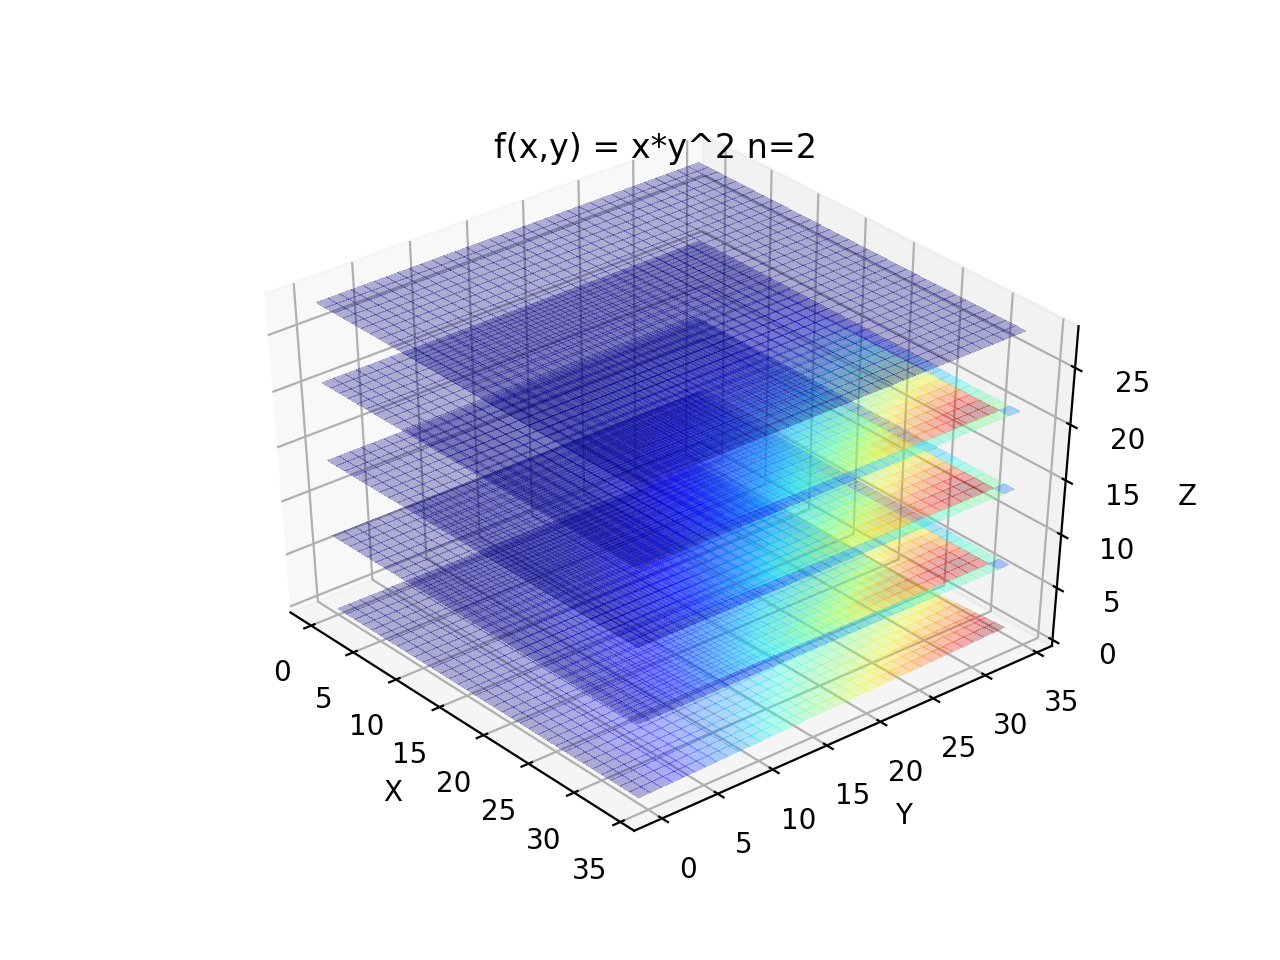
\includegraphics[width=1.5in]{images/xy2-n2}
  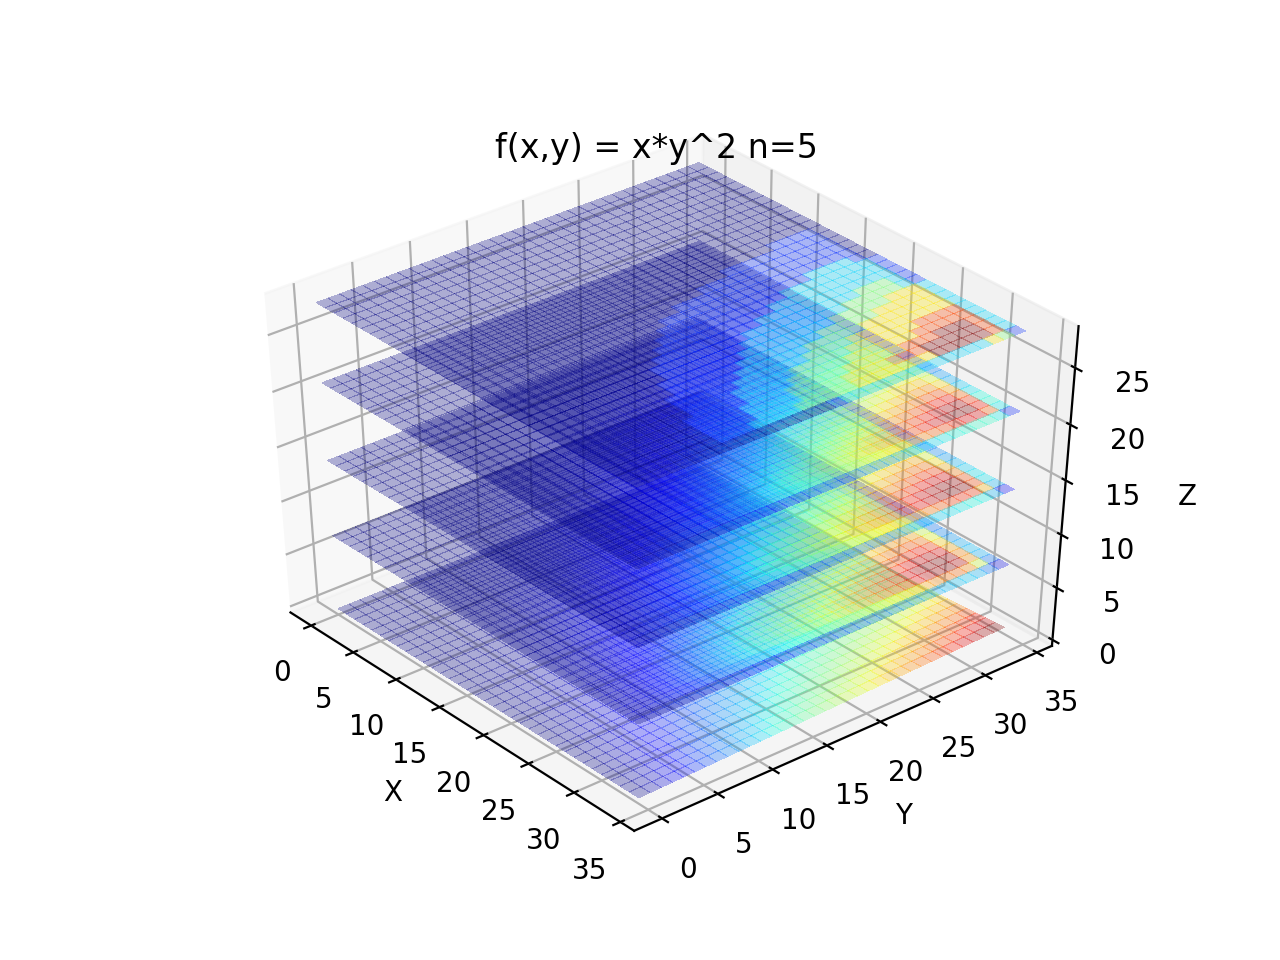
\includegraphics[width=1.5in]{images/xy2-n5}
  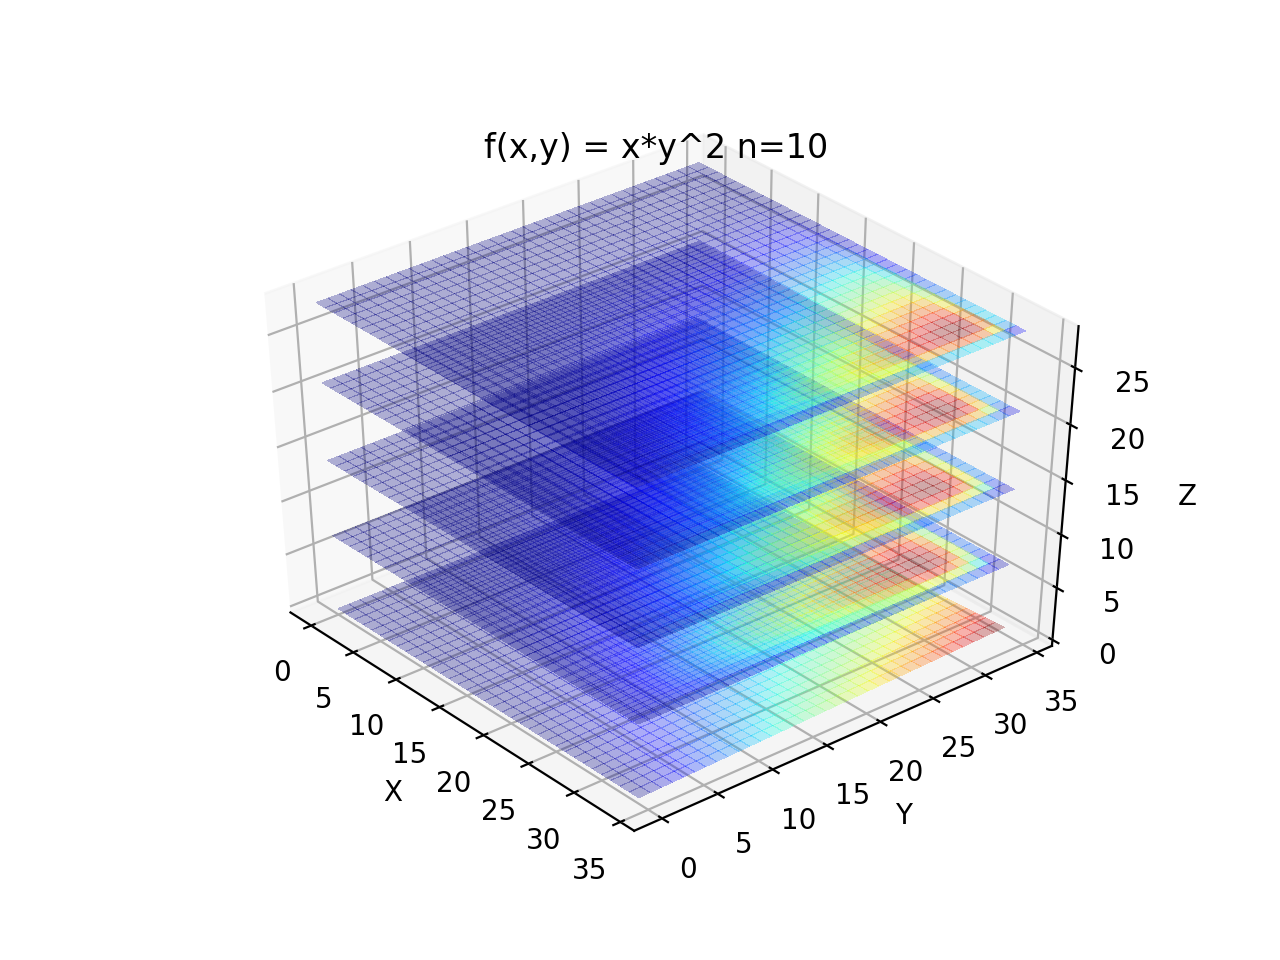
\includegraphics[width=1.5in]{images/xy2-n10}
  \caption{\(h(y) = g(y) = 2y^3+5\) con iteraciones \(n = 0, 2, 5 \text{ y } 10\)}
  \label{xy2-iterations}
\end{figure}


\subsection{Ecuación de Laplace en coordenadas esféricas}



\section{Conclusion}
The conclusion goes here.





% if have a single appendix:
%\appendix[Proof of the Zonklar Equations]
% or
%\appendix  % for no appendix heading
% do not use \section anymore after \appendix, only \section*
% is possibly needed

% use appendices with more than one appendix
% then use \section to start each appendix
% you must declare a \section before using any
% \subsection or using \label (\appendices by itself
% starts a section numbered zero.)
%


\appendices
\section{Proof of the First Zonklar Equation}
Appendix one text goes here.

% you can choose not to have a title for an appendix
% if you want by leaving the argument blank
\section{}
Appendix two text goes here.


% use section* for acknowledgment
\ifCLASSOPTIONcompsoc
  % The Computer Society usually uses the plural form
  \section*{Acknowledgments}
\else
  % regular IEEE prefers the singular form
  \section*{Acknowledgment}
\fi


The authors would like to thank...


% Can use something like this to put references on a page
% by themselves when using endfloat and the captionsoff option.
\ifCLASSOPTIONcaptionsoff
  \newpage
\fi



% trigger a \newpage just before the given reference
% number - used to balance the columns on the last page
% adjust value as needed - may need to be readjusted if
% the document is modified later
%\IEEEtriggeratref{8}
% The "triggered" command can be changed if desired:
%\IEEEtriggercmd{\enlargethispage{-5in}}

% references section

% can use a bibliography generated by BibTeX as a .bbl file
% BibTeX documentation can be easily obtained at:
% http://mirror.ctan.org/biblio/bibtex/contrib/doc/
% The IEEEtran BibTeX style support page is at:
% http://www.michaelshell.org/tex/ieeetran/bibtex/
%\bibliographystyle{IEEEtran}
% argument is your BibTeX string definitions and bibliography database(s)
%\bibliography{IEEEabrv,../bib/paper}
%
% <OR> manually copy in the resultant .bbl file
% set second argument of \begin to the number of references
% (used to reserve space for the reference number labels box)
\begin{thebibliography}{1}

\bibitem{IEEEhowto:kopka}
H.~Kopka and P.~W. Daly, \emph{A Guide to \LaTeX}, 3rd~ed.\hskip 1em plus
  0.5em minus 0.4em\relax Harlow, England: Addison-Wesley, 1999.

\end{thebibliography}

% biography section
% 
% If you have an EPS/PDF photo (graphicx package needed) extra braces are
% needed around the contents of the optional argument to biography to prevent
% the LaTeX parser from getting confused when it sees the complicated
% \includegraphics command within an optional argument. (You could create
% your own custom macro containing the \includegraphics command to make things
% simpler here.)
%\begin{IEEEbiography}[{\includegraphics[width=1in,height=1.25in,clip,keepaspectratio]{mshell}}]{Michael Shell}
% or if you just want to reserve a space for a photo:

\begin{IEEEbiography}{Michael Shell}
Biography text here.
\end{IEEEbiography}

% if you will not have a photo at all:
\begin{IEEEbiographynophoto}{John Doe}
Biography text here.
\end{IEEEbiographynophoto}

% insert where needed to balance the two columns on the last page with
% biographies
%\newpage

\begin{IEEEbiographynophoto}{Jane Doe}
Biography text here.
\end{IEEEbiographynophoto}

% You can push biographies down or up by placing
% a \vfill before or after them. The appropriate
% use of \vfill depends on what kind of text is
% on the last page and whether or not the columns
% are being equalized.

%\vfill

% Can be used to pull up biographies so that the bottom of the last one
% is flush with the other column.
%\enlargethispage{-5in}



% that's all folks
\end{document}


